%:Clase del documento
\documentclass[paper=a4,10pt, Myfinal=true,twoside]{scrbook}
%Minion=true, English=true, Myfinal=true

%:Paquete de estilos propuesto
\usepackage{libroETSI}

%:Paquete específico para cargar tikz (y sus librerías) y pgfplots
\usepackage{dtsc-creafig}

%:Paquete para notaciones específicas
\usepackage{notacion}

%:Paquete para incorporar aspectos concretos de la edición
\usepackage{edicionPFC}


%:Estas líneas de código son INNECESARIAS excepto para mostrar determinadas características en este manual. Pueden eliminarse o comentarse sin ningún problema.
%Se usan para compilar el capítulo estilolibroetsi.tex
\usepackage[final]{showexpl}
\lstset{explpreset={frame=none,rframe={}, numbers=none,numbersep=3pt, columns=flexible,language={[LaTeX]TeX},basicstyle=\ttfamily,keywordstyle=\color{blue}}}%numberstyle=\tiny,

%:Para modificar fácilmente la fuente del texto.
\makeatletter
\ifdtsc@Minion % Queremos utilizar la fuente Minion y lo hemos declarado al principio
	\ifluatex
		\setmainfont[Renderer=Basic, Ligatures=TeX,	% Fuente del texto 
		Scale=1.01,
		]{Minion Pro}
   		% En este caso conviene modificar ligeramente el tamaño de las fuentes matemáticas
		\DeclareMathSizes{10}{10.5}{7.35}{5.25}
		\DeclareMathSizes{10.95}{11.55}{8.08}{5.77}
		\DeclareMathSizes{12}{12.6}{8.82}{6.3}
%		\setmainfont[Renderer=Basic, Ligatures=TeX,	% Fuente del texto 
%		]{Adobe Garamond Pro}
%		\setmainfont[Renderer=Basic, Ligatures=TeX,	% Fuente del texto 
%		]{Palatino LT Std}
	\fi
\else
	\ifluatex
		% Para utilizar la fuente Times New Roman, o alguna otra que se tenga instalada
		\setmainfont[Renderer=Basic, Ligatures=TeX,	% Fuente del texto 
		Scale=1.0,
		]{Times New Roman}
	\else
		\usepackage{tgtermes} 	%clone of Times
		%\usepackage[default]{droidserif}
		%\usepackage{anttor} 	
	\fi
\fi
\makeatother

%Por si quieren usar bibliografía con BIBER
%BIBER%%:Para la bibliografía en BIBER, descomentar las líneas siguientes
%\defbibheading{etsi}[]{%
%	\chapter*{Bibliografía}%
%	\chaptermark{Bibliografía} 
%	\markboth{#1}{#1}}
%\addbibresource{bibliografiaLibroETSI.bib}

% Ejemplo de Glosario
\newacronym[type=main]{DoS}{DoS}{Denial of Service}
\newacronym[type=main]{DDoS}{DDoS}{Distributed DoS}
\newacronym[type=main]{IP}{IP}{Internet Protocol}
\newacronym[type=main]{TCP}{TCP}{Transmission Control Protocol}
\newacronym[type=main]{UCP}{UCP}{User Datagram Protocol}
\newacronym[type=main]{ICMP}{ICMP}{Internet Control Message Protocol}
\newacronym[type=main]{ITU-T}{ITU-T}{International Telecommunications Union}
\newacronym[type=main]{CNSS}{CNSS}{Committee on National Security Systems}
\newacronym[type=main]{PFRING}{PFRING}{Packet Filter RING}
\newacronym[type=main]{API}{API}{Application Programming Interface}
\newacronym[type=main]{NAPI}{NAPI}{New API, nueva API}


\makeindex
\makeglossaries %Si no se quiere el glosario, comentar esta línea.

% Formato A4
\geometry
{paperheight=297mm,%
paperwidth=210mm,%
top=25mm,%
headsep=8.5mm,%
includefoot, 
textheight=240mm, 
textwidth=150mm, 
bindingoffset=0mm, 
twoside}

\usepackage[a4,center]{crop}%para poner las cruces de esquina de página, poner la opción cross

%:Esquema de numeración por defecto
\setenumerate[1]{label=\normalfont\bfseries{\arabic*.}, leftmargin=*, labelindent=\parindent}
\setenumerate[2]{label=\normalfont\bfseries{\alph*}), leftmargin=*}
\setenumerate[3]{label=\normalfont\bfseries{\roman*.}, leftmargin=*}
\setlist{itemsep=.1em}
\setlength{\parindent}{1.0 em}

\setcounter{tocdepth}{4}  % El nivel hasta el que se muestra el índice 
\newcommand{\redborderddos}{RedBorder DDoS}


%:Empieza el documento

\begin{document}
%:Para incluir toda la referencia bibliográfica aunque no se cite, descomente la siguiente línea
%\nocite{*}


%PORTADA
%ver edicionPFC.sty para modificaciones

% @TODO ttitulo
%:Para crear la portada y la portada interior (pagina titular)
\titulo{Formato de Publicación de la Escuela \mbox{Técnica} Superior de Ingeniería} %\mbox evita que se divida una palabra al cambiar de línea
\autor{Eugenio Pérez Martín}
\director{Pablo Nebrera Herrera}
\titulodirector{Profesor Asociado}

\departamento{Departamento de Ingeniería Telemática}
\centro{Escuela Técnica Superior de Ingeniería}
\universidad{Universidad de Sevilla}
\titulacion{Ingeniería de Telecomunicación}
\fecha{2014}
\nombretrabajo{Proyecto Fin de Grado} %Trabajo Fin de Grado, Proyecto fin de Máster,....

\hypersetup
	{
 	linkcolor=black, %Tocar para poner color en enlaces
	pdfauthor={\elautor},
	pdftitle={\nombretrabajo,\eltitulo}, 
	pdfkeywords={Latex, edición, formato de texto}	
	 }

 %logo de la Universidad y logo del departamento, si lo hubiera. Para cambiar el pie de página con 
% los logos, debe editarse el fichero ediciónPFC.sty

\portadaPFC{figuras/LogoUS.pdf}{figuras/LogoDIT.pdf}

%Fin Portada

%:Todo lo que constituye la primera parte del libro que no es el cuerpo del libro en realidad
\frontmatter
\pagenumbering{Roman} %Pone la numeración en mayúscula (En español parece que es obligatorio)

%\include{dedicatoria/dedicatoria}%¿Comentar para proyectos/tesis?
% !TEX root =../LibroTipoETSI.tex
\chapter*{Agradecimientos}
%\pagestyle{especial}
\pagestyle{empty}
%\chaptermark{Agradecimientos}
\phantomsection
%\addcontentsline{toc}{listasf}{Agradecimientos}
%\vspace{1cm}
%{\huge{Agradecimientos}}
%\vspace{1cm}

\lettrine[lraise=-0.1, lines=2, loversize=0.25]{E}{l} diseño de una hoja de estilo en \LaTeX\ para un texto no es en absoluto trivial. Por un lado hay que conocer bien los usos, costumbres y reglas que se emplean a la hora de establecer márgenes, tipos de letras, tamaños de las mismas, títulos, estilos de tablas, y un sinfín de otros aspectos. Por otro, la programación en \LaTeX\ de esta hoja de estilo es muy tediosa, incluida la selección de los mejores paquetes para ello. La hoja de estilo adoptada por nuestra Escuela y utilizada en este texto es una versión de la que el profesor Payán realizó para un libro que desde hace tiempo viene escribiendo para su asignatura. Además, el prof. Payán ha participado de forma decisiva en la adaptación de dicha plantilla a los tres tipos de documentos que se han tenido en cuenta: libro, tesis y proyectos final de carrera, grado o máster. Y también en la redacción de este texto, que sirve de manual para la utilización de estos estilos. Por todo ello, y por hacerlo de forma totalmente desinteresada, la Escuela le está enormemente agradecida.

A esta hoja de estilos se le incluyó unos nuevos diseños de portada. El diseño gráfico de las portadas para proyectos fin de grado, carrera y máster, está basado en el que el prof. Fernando García García, de la Facultad de Bellas Artes de nuestra Universidad, hiciera para los libros, o tesis, de la sección de publicación de nuestra Escuela. Nuestra Escuela le agradece que pusiera su arte y su trabajo, de forma gratuita, a nuestra disposición.

%gradecemos}, a todos nuestros maestros, cuanto nos enseñaron.

{\flushleft{\hfill \emph{Juan José Murillo Fuentes}}}%
\vspace{-.3cm}
{\flushleft{\hfill \emph{Subdirección de Comunicaciones y Recursos Comunes}}}%
{\flushleft{\hfill \emph{Sevilla, 2013}}}%

%PFC/PFM/TESIS
% !TEX root =../LibroTipoETSI.tex
\chapter*{Resumen}
\pagestyle{especial}
\chaptermark{Resumen}
\phantomsection
\addcontentsline{toc}{listasf}{Resumen}

\lettrine[lraise=-0.1, lines=2, loversize=0.2]{E}{n} nuestra Escuela se producen un número considerable de documentos, tantos docentes como investigadores. Nuestros alumnos también contribuyen a esta producción a través de sus trabajos de fin de grado, máster y tesis. El objetivo de este material es facilitar la edición de todos estos documentos y a la vez fomentar nuestra imagen corporativa, facilitando la visibilidad y el reconocimiento de nuestro Centro.

%La hoja de estilo utilizada es una versión de la que el Prof. Payán realizó para un libro que desde hace tiempo viene escribiendo para su asignatura. Con ella se han realizado estas notas, a modo de instrucciones, añadiéndole el diseño de la portada. El diseño de la portada está basado en el que el prof. Fernando García García, de nuestra universidad, hiciera para los libros de la sección de publicación de nuestra Escuela.


\chapter*{Abstract}
\pagestyle{especial}
\chaptermark{Abstract}
\phantomsection
\addcontentsline{toc}{listasf}{Abstract}

\lettrine[lraise=-0.1, lines=2, loversize=0.2]{I}{n} our school there are a considerable number of documents, many teachers and researchers. Our students also contribute to this production through its work in order of degree, master's theses. The aim of this material is easier to edit these documents at the same time promote our corporate image, providing visibility and recognition of our Center. 

...
\emph{-translation by google-}

 

% Índice abreviado 
% El índice abreviado se incluye también en algunos libros, con menor detalle que el completo. Descomentar las siguientes líneas.
\cleardoublepage
\phantomsection
\addcontentsline{toc}{listasf}{Índice Abreviado}
\pagestyle{especial}
\shorttoc{Índice Abreviado}{1}

%Índice normal, el completo
\cleardoublepage
\phantomsection
\pagestyle{especial}
\tableofcontents


% \chapter*{\notationname}
\pagestyle{especial}
\chaptermark{\notationname}
\phantomsection
\addcontentsline{toc}{listasf}{\notationname}
%\section*{Notación}
%\begin{table}[htbp]
\begin{longtable}{p{3cm}p{8.5cm}}

%$\displaystyle D$ & Tasa de símbolos  (sim/s) \\
%$\displaystyle R_b$ & Tasa binaria (bit/s) \\
%$\displaystyle T$ & Tiempo de símbolo (s) \\
%$\displaystyle T_{b}$ & Tiempo de bit (s) \\
%$W\left( {t} \right)$ & Ruido blanco\\
%$w\left( {t} \right)$ & Función muestra de un ruido blanco\\
%$\displaystyle h_{c}\left( {t} \right)$ & Respuesta impulsiva de un canal LTI continuo en el tiempo\\
%$\displaystyle H_{c}\left( {\omega} \right)$ & Respuesta en frecuencia de un canal LTI continuo en el tiempo\\
%$\displaystyle h_{c}\left( {\tau;t} \right)$ & Respuesta impulsiva de un canal LTV continuo en el tiempo\\
%$\displaystyle H_{c}\left( {\omega;t} \right)$ & Respuesta en frecuencia de un canal LTV continuo en el tiempo\\
%$\displaystyle h_{c}\left( {n} \right)$ & Respuesta impulsiva de un canal LTI discreto en el tiempo\\
%$\displaystyle H_{c}\left( {\Omega} \right)$ & Respuesta en frecuencia de un canal LTI discreto en el tiempo\\
$\RR$ & Cuerpo de los números reales \\
$\CC$ & Cuerpo de los números complejos\\
$\left\| \vc{v} \right\|$ & Norma del vector $\vc{v}$ \\
$\left\langle {\vc{v}, \vc{w}} \right\rangle$ & Producto escalar de los vectores $\vc{v}$ y $\vc{w}$\\
$\left| {\vc{A}} \right|$ &Determinante de la matriz cuadrada $\vc{A}$\\
$\textrm{det}\left( {\vc{A}} \right)$ &Determinante de la matriz (cuadrada) $\vc{A}$\\
$\vc{A}\trs$ & Transpuesto de $\vc{A}$\\
$\vc{A}\inv$ & Inversa de la matriz $\vc{A}$\\
$\vc{A}{\psd}$ & Matriz pseudoinversa de la matriz $\vc{A}$\\
$\vc{A}\her$ & Transpuesto  y conjugado de $\vc{A}$\\
$\vc{A}\cnj$ & Conjugado\\
c.t.p. & En casi todos los puntos\\
c.q.d. & Como queríamos demostrar\\
\ensuremath{\blacksquare}& Como queríamos demostrar\\
\ensuremath{\square}& Fin de la solución\\
e.o.c. & En cualquier otro caso\\
$\e$ & número e\\
$\xp{x}$ & Exponencial compleja\\
$\xppi{x}$ & Exponencial compleja con $2\pi$\\
$\nxp{x}$ & Exponencial compleja negativa\\
$\nxppi{x}$ & Exponencial compleja negativa con $2\pi$\\
$\re$ & Parte real\\
$\im$ & Parte imaginaria\\
$\sen$ & Función seno \\
$\tg$ & Función tangente \\
$\arctg$ & Función arco tangente \\
$\sento{y}{x}$ & Función seno de $x$  elevado a $y$\\
$\costo{y}{x}$ & Función coseno de $x$  elevado a $y$\\
$\sa$ & Función sampling \\
$\sgn$ & Función signo \\
$\rect$ & Función rectángulo \\
$\sinc$ & Función sinc\\
$\pder{y}{x} $ & Derivada parcial de $y$ respecto a $x$\\
$x\gra$ & Notación de grado, $x$ grados.\\
%
%$C_{XY}$& covarianza  de dos variables aleatorias reales $X$ e $Y$\\
%$R_{XY}$& correlación  de dos variables aleatorias reales $X$ e $Y$\\
%$\rho_{XY}$ &Coeficiente de correlación de las variables aleatorias reales $X$  e $Y$\\
%$\vc{Z}$ & Vector aleatorio complejo\\
%$\displaystyle F_{X}\left( {\cdot} \right)$ & Función de distribución de la variable aleatoria $X$ \\
%$\displaystyle f_{X}\left( {\cdot} \right)$ & Función densidad de probabilidad de la variable aleatoria $X$ \\
%$p_{X}\left( {\cdot} \right)$ & Función masa de probabilidad de la variable aleatoria discreta $X$ \\
%
$\Pr\left( {A} \right)$ & Probabilidad del suceso $A$ \\
$\displaystyle E\left[ {X} \right]$ & Valor esperado de la variable aleatoria $X$ \\
$\si{X}$ & Varianza de la variable aleatoria $X$\\
$\sim f_{X}\left( {x} \right)$ & Distribuido siguiendo la función densidad de probabilidad $f_{X}\left( {x} \right)$\\
%
$\gauss{m_{X}}{\si{X}}$ &Distribución gaussiana para la variable aleatoria X, de media $m_{X}$ y varianza $\si{X}$ \\
$\id{n}$ & Matriz identidad de dimensión $n$\\
$\diag{\vc{x}}$ & Matriz diagonal a partir del vector $\vc{x}$\\
$\diag{\vc{A}}$ & Vector diagonal de la matriz $\vc{A}$\\
$\snr$& Signal-to-noise ratio \\
$\mse$ & Minimum square error\\
$\talq$ & Tal que \\
$\eqdef$ & Igual por definición \\
$\norm{\vc{x}}$ & Norma-2 del vector $\vc{x}$\\
$\card{\vc{{A}}}$ & Cardinal, número de elementos del conjunto $\vc{A}$\\
$\xyz{\vc{x}}{i}{n}$ & Elementos $i$, de 1 a $n$, del vector $\vc{x}$\\
%\newcommand{\xyz}[3]{\ensuremath{#1_{#2},#2=1,2,\ldots,#3}}
$\df{x}$& Diferencial de $x$\\
$\le$ & Menor o igual \\
$\ge$ & Mayor o igual \\
$\BL$ & Backslash \\
$\iff$ & Si y sólo si \\
$x=a+3\eqexpl{a=1} 4 $& Igual con explicación \\
$\tfrac{a}{b}$ & Fracción con estilo pequeño, $a/b$ \\
$\inc$ & Incremento \\
$b\ten{a}$ & Formato científico \\
$\tendsub{x}$ & Tiende, con x \\
$\ord$ & Orden\\
$\tm$ & Trade Mark\\
$\E[x]$ & Esperanza matemática de x\\
$\covm{\vc{x}}$ & Matriz de covarianza de $\vc{x}$\\
$\corrm{\vc{x}}$ & Matriz de correlación de $\vc{x}$\\
$\si{x}$ & Varianza de x \\


\end{longtable}
\newpage
%\end{table}
%


%\phantomsection
%\addcontentsline{toc}{listasf}{Acrónimos}
%\section*{Acrónimos}
%\begin{table}[htbp]
%\begin{tabular}{p{2cm}p{10cm}}
%Escuela Técnica Superior de In
%LTI & Lineal Invariante con el Tiempo \\
%LTV& Lineal Variable con el Tiempo\\
%AWGN& Ruido blanco gaussiano aditivo\\
%DMS& Fuente discreta sin memoria\\
%AEP& Propiedad de equipartición asintótica\\
%WLLN& Ley Débil de los Grandes Números\\
%DMC& Canal Discreto sin Memoria\\
%BSC& Canal Simétrico Binario\\
%BEC& Canal Binario con Borrado\\
%\end{tabular}
%\end{table}


%\nota{El libro de Lapidoth tiene una excelente recopilación.} %No incluir si no se quiere, comentándolo

%:Empieza el contenido del libro
\mainmatter

%:Página por defecto
\pagestyle{esitscCD}

%:Los diferentes capítulos, en carpetas separadas
% TODO prefacio
%
% !TEX root =../LibroTipoETSI.tex
%El anterior comando permite compilar este documento llamando al documento raíz
\chapter{Guía de Uso}\label{chp-01}
\epigraph{The fundamental problem of communication is that of reproducing at one point either exactly or approximately a message selected at another point.}{Claude Shannon, 1948}

%\lettrine[lraise=0.7, lines=1, loversize=-0.25]{E}{n}
\lettrine[lraise=-0.1, lines=2, loversize=0.2]{E}{n} este capítulo vamos a describir las partes de las que consta un documento tipo, cómo deben interpretarse los diferentes comandos que se han definido para su confección, los \indexit{paquetes} (conjunto de sentencias de \LaTeX\ escritas y desarrolladas por diversos autores) que se han cargados y el porqué de los mismos, elecciones realizadas en cuanto a la edición, el porqué de determinadas fuentes, etc. 

Hay mucho de elección personal en lo que sigue y únicamente se justifica desde el gusto personal de quienes escribimos esto. No pretendemos por ello sentar precedentes, obligaciones ni restricciones a quien desee utilizar este documento. En cualquier caso, esperamos que su lectura sea provechosa para la confección y edición de libros, apuntes de clase, proyectos, etc.

\LaTeX se ha convertido de hecho en el procesador de texto estándar para la edición de documentos científicos. Este libro está escrito precisamente en \LaTeX, haciendo uso de la plantilla que hemos diseñado y al escribir un libro sobre cómo escribir un libro en \LaTeX\  y cómo hacer uso de esta plantilla, estamos entrando muchas veces en una redundancia evidente.

Estas páginas no constituyen un manual de \LaTeX,  ni lo pretendemos, ya que existen incontables y buenas referencias sobre este tema. El objetivo es describir los aspectos formales que deseamos se puedan incorporar a cualquier texto producido en la Escuela.  También, como la mayoría de nuestra producción científica utiliza ampliamente las fórmulas matemáticas, incluimos algunos consejos sobre la escritura de las mismas, para lo que hemos utilizado las notas preparadas en \cite{moser}. Asimismo resulta muy interesante el libro \cite{gratzer}.

Por último, puesto que los ficheros fuentes de este documento están disponibles, esperamos que los mismos faciliten la utilización de los distintos elementos de edición.

\section{Cómo usar los  estilos de documento de la ETSI}\label{sec-00}

Una de las bondades del \LaTeX\ es que una vez definido el estilo, formado por un conjunto de paquetes y adaptaciones de los mismos, la escritura de un texto se reduce a dominar una serie de comandos. En nuestro caso, se presenta este documento como ejemplo de uso de estos comandos. En este capítulo encontrará detalles técnicos sobre la estructura del documento y una breve introducción sobre algunos de los elementos del estilo diseñado, puesto que en el Capítulo \ref{chap:estilo} se estudian detalladamente todos sus componentes. También encontrará instrucciones de cómo compilar el documento. Para usar esta hoja de estilo, se recomienda leer el Capítulo \ref{chap:CAPEJ} y Capítulo \ref{chap:CAPPB} como ejemplos de capítulos donde se incluyen la mayoría de los comandos que pueden ser de utilidad en la redacción de un texto técnico. 

El archivo \ttcolor{libroTipoETSI.tex} es el archivo principal, que tiene una serie de comandos para incluir las distintas partes que se necesiten. Muchas de estas partes se han incluido separadamente en carpetas, por comodidad. Este archivo lo hemos modificado levemente para utilizarlo como formato para proyecto fin de carrera/grado/máster. El resultado se incluye en un fichero con nombre \ttcolor{pfcTipoETSI.tex}. Y también se incluye un formato para tesis \ttcolor{tesisTipoETSI.tex}

Los datos necesarios para generar la cubierta y demás hojas iniciales se incluyen al comienzo de estos ficheros: el título del proyecto, autores, el nombre del departamento, etc. Si necesita retocar la cubierta  (por ejemplo el ancho de la imagen utilizada)  tendrá que modificar directamente el fichero \ttcolor{edicionLibro.sty}, que es el fichero al que se llama para generarla. Si quiere, también, puede retocar la imagen de fondo. Todo esto se explica en un apartado más adelante. Para los restantes tipos de documentos, estas modificaciones hay que hacerlas en los ficheros \ttcolor{edicionPFC.tex} y \ttcolor{edicionTesis.sty}.

Así, para empezar a utilizar este documento, basta que empiece modificando los ficheros \ttcolor{libroTipoETSI.tex} (ó \ttcolor{pfcTipoETSI.tex}, {tesisTipoETSI.tex} ) y cada uno de los ficheros que éste incluya, bien introduciendo los cambios oportunos, bien eliminándolos (puede simplemente comentar la línea correspondiente).

Una vez modificado, el segundo paso es compilarlo. Debe elegir el tipo de formato, A4 ó libro. Por defecto, \ttcolor{libroTipoETSI.tex} y \ttcolor{tesisTipoETSI.tex}  están en formato libro y \ttcolor{pfcTipoETSI.tex} en A4. Para cambiar cualquiera de ellos, debe buscar el comando \ttcolorc{geometry} dentro del fichero  \ttcolor{libroTipoETSI.tex} y establecer los parámetros correspondientes o bien tendrá que comentar la correspondiente a tamaño libro para descomentar la correspondiente al formato A4, o viceversa. También, hay un conjunto de comandos más adelante que están comentados y que permiten presentar el texto en formato \ind{manuscrito}, con un interlineado distinto prefijado a $1.5$ líneas. 

\subsection{Compilación}

\subsubsection{{Macintosh}\tsp{\textregistered}}
Este trabajo se ha desarrollado en un ordenador \ind{Macintosh}\tsp{\textregistered}. Como iremos viendo, \LaTeX\ consta de un elevado número de programas y existen un conjunto de distribuciones que facilitan su uso. Nosotros hemos elegido una de las versiones más utilizadas, Tex-Live, versión 2013, \url{http://mirror.ctan.org/systems/mac/mactex/MacTeX.pkg}, en su versión para el sistema operativo Mac OSx\tsp{\textregistered}. Para la bibliografía  se ha utilizado \ind{BibTex}. 

Como editor de ficheros y compilador hemos usado \ind{TeXShop}\tsp{\textregistered}. Puede usar pdflatexmk para compilar, que va bien y genera directamente la bibliografía y los índices de palabra y glosarios. Aquí se recomienda utilizar el comando \ttcolor{lualatexmk}, que es un determinado motor \ind{engine} de TeXShop\tsp{\textregistered}. Si no lo ve en la lista de opciones de componer, vaya a las librerías de usuario y en la carpeta TeXShop/Engines saque lualatexmk.engine de la subcarpeta Inactive. Si no quiere complicarse,  En todo caso, puede usar también \LaTeX\ y BibTeX. Pero si compila con \LaTeX\ y luego desea usar Lua\LaTeX mk, deberá borrar todos los archivos auxiliares, menos los archivos con la extensión \ttcolor{.tex} y \ttcolor{.bib} que se corresponden, respectivamente, al fichero fuente de \LaTeX\ y de la bibliografía.

Si utiliza un índice de palabras y un glosario, vaya a la sección correspondiente para ver cómo generarlos.

\subsubsection{Windows\tsp{\textregistered}}

Existen versiones de la distribución Tex-Live para las diferentes versiones de Windows\tsp{\textregistered} y en la dirección señalada anteriormente pueden encontrarse instrucciones para su instalación en este y restantes sistemas operativos. No se ha probado con el conjunto MikTeX, pero probablemente funcionaría igualmente.

Como editor y compilador de ficheros hemos optado por \ind{TexMaker}\tsp{\textregistered}, igualmente con una codificación UTF-8. Hasta donde conocemos, el editor \indexit{Winedt}\tsp{\textregistered} no reconoce esta codificación. Para la bibliografía se ha utilizado BibTeX. Para compilar tendrá que o bien usar LatexMk ó PDFLaTeX. No olvide seleccionar la opción UTF-8 en ``Opciones'' en el menú, y luego en la ventana emergente pulsando Editor y allí en el campo Codificación de editor. 

Si utiliza un índice de palabras y un glosario, vaya a la sección correspondiente para ver cómo generarlos.

\subsubsection{Lyx}

En \url{http://www.lyx.org/}, el lector puede encontrar una opción alternativa a la forma de trabajo tradicional de \LaTeX, tanto en Windows\tsp{\textregistered} como en MacOS\tsp{\textregistered}. En este entorno, uno puede trabajar con un entorno de edición gráfico, tal como se trabaja por ejemplo en Microsoft Word\tsp{\textregistered}. Una vez terminado el documento, es relativamente sencillo compilarlo en \LaTeX. De hecho, hemos realizado algunas pruebas positivas en este sentido. En cualquier caso se recomienda no usar nombres de archivo con ñ, tildes, o espacios. 

\subsection{Texto en inglés}
Si escribe el texto en inglés, deberá de cambiar el idioma en la opción de Babel, uno de los paquetes claves para la escritura en \LaTeX. En el fichero \ttcolor{libroTipoETSI.sty}, se debe buscar la línea que comienza por \comando{usepackage}\ttcolor{[spanish, english...]\{babel\} } y seguir con las instrucciones correspondientes. Esto hará que automáticamente los nombres de secciones, apartados, teoremas, ejemplos, etc, aparezcan en inglés. 

\section{Elementos básicos de un libro}
%
En este capítulo describimos los puntos que pueden incluirse con el formato propuesto. En primer lugar, la longitud de un libro, en general, justifica su separación en partes. Una posibilidad es que un libro esté dividido en Partes y esta a su vez en Capítulos. Y por último, a veces existen Apéndices que se incorporan cuando han acabado los capítulos. En nuestro caso sólo hemos considerado la posibilidad de dividir el libro en capítulos y apéndices. Además, existen un conjunto de elementos como dedicatoria, prefacio, agradecimientos, portada, etc, que también son partes que se han tenido en cuenta. 

Se ha optado por estructurar los ficheros fuente de este texto en carpetas que cuelgan de una principal en la que se encuentra alojada el fichero principal que las utiliza o agrupa. En nuestro caso, por ejemplo, el fichero principal se denomina \ttcolor{libroTipoETSI.tex} (ó \ttcolor{pfcTipoETSI.tex}, \ttcolor{tesisTipoETSI.tex}) y colgadas de la carpeta que lo contiene se encuentran las carpetas \ttcolor{introducción}, \ttcolor{dedicatoria}, ..., \ttcolor{capitulolibroETSI}\footnote{Tenga en cuenta que en algunas imprentas pueden cobrar más por copias de hojas en color. Para ello asegúrese de que utiliza los colores convenientemente, y -en su caso- que los grises lo son de verdad.}, etc. De alguna forma, este fichero principal es el esqueleto que describe cómo está formado el libro.

En un nivel de descripción diferente, podríamos considerar que un libro se encuentra dividido en cubierta, páginas de cortesía, portada, página de título y trasera de la página de título, elementos antes del cuerpo del libro, tales como agradecimientos, prefacio, índices, etc, el cuerpo del libro en sí, dividido en capítulos y esto a su vez en secciones, subsecciones, subsubsecciones, %parágrafos,
subcapítulos, apéndices y, por último, la parte del libro después del cuerpo, que agruparía elementos tales cómo la lista de figuras del libro, la bibliografía, el índice, etc. En \LaTeX\ estas tres partes se dividen con los comandos  \ttcolorc{frontmatter}, \ttcolorc{mainmatter} y \ttcolorc{backmatter}. Estos comandos, y muchos otros, nos permiten describir formalmente el contenido del libro, tal cómo se realiza en el fichero \ttcolor{libroTipoETSI.tex}. Este fichero, como hemos dicho, constituye el esquema de nuestro libro y entender por qué están allí cada una de sus partes es de interés, que no imprescindible, de cara a poder confeccionar un texto. 
%Veamos sus diferentes partes.

\section{Clase de documento}
El comando \comandos{documentclass[paper=a4,10pt, twoside]}{scrbook} o uno similar es el primer comando que aparecerá en cualquier documento de \LaTeX. La parte importante del mismo es \ttcolor{scrbook} y hace referencia a la elección de una  clase de documento tipo libro pero tal como se define en el conjunto de programas denominado \ttcolor{Koma}. Se ha elegido este tipo de documento fundamentalmente por generar un tipo de texto próximo a los estándares europeos, en contraposición con la clase estándar \ttcolor{book}. Una posible alternativa consistiría en la utilización de la clase \ttcolor{Memoir}. En cualquier caso, debido a las posibles modificaciones del conjunto \ttcolor{Koma}, es inmediato sustituir la clase de documento por la standard \ttcolor{book}.

Existen además un conjunto de parámetros, todos los encerrados entre \ttcolor{[...]} que modifican de alguna manera el tipo de documento que vamos a generar. Para entender el significado de cada uno de ellos se puede consultar la referencia \cite{koma}. En cualquier caso, \ttcolor{paper=a4} hace referencia a la dimensión del papel que vamos a utilizar (más adelante diremos algo más acerca de esto), \ttcolor{10pt} establece el tamaño de la fuentes en \ttcolor{puntos tipográficos} y \ttcolor{twoside} nos indica que vamos a generar un documento a doble cara. 

Por último, se han incorporado tres nuevos parámetros: \ttcolor{Myfinal=false}, \ttcolor{Minion=false} y \ttcolor{English=false}. Mediante el primero, que como todos ellos también puede tomar el valor \ttcolor{Myfinal=true}, se le indica a \LaTeX\ que nos encontramos en la versión final del documento, realizándose con ello una serie de ajustes \emph{finos} en la partición silábica, la separación entre palabras (o incluso un ligero ensanchamiento) que hacen más agradable visualmente el texto generado. 

Mediante el parámetro \ttcolor{Minion=true} ó \ttcolor{Minion=false} se le indica a  \LaTeX\ que utilice o no el paquete \ttcolor{Minion}. Este paquete permite la utilización de una fuente denominada Minion Pro para el texto y el conjunto de símbolos matemáticos que lo acompañan, denominados MnSymbol. No resulta trivial la instalación de este paquete por lo que en general la opción por defecto es su no utilización. No hay que confundir la utilización de la opción \ttcolor{Minion=true} ó \ttcolor{Minion=false} con el uso de la fuente Minion Pro para el texto del documento. Ambas cosas están separadas aunque desde un punto de vista tipográfico no deberían estarlo. Es decir, si queremos elegir una fuente Minion Pro para el texto, lo más acertado sería elegir esa misma fuente para el texto matemático. Esta elección conjunta es la que se activa con \ttcolor{Minion=true}.

Por último, resulta evidente el significado  del parámetro \ttcolor{Englis=false} que también puede ser \ttcolor{English=true}.

\section{Fichero de estilo LibroETSI.sty}
La instrucción que sigue a la declaración de la clase es  \comandos{usepackage}{LibroETSI}. Con ella  cargamos y definimos  las principales características tipográficas y de muy diversa índole que hemos propuesto para el diseño de los documentos de la Escuela. A lo largo del presente documento se irán revelando diversos aspectos del mismo, pero se empieza aquí con una pequeña introducción. En el Capçitulo correspondiente se describen ordenadamente todas sus características. 

Debemos observar antes que nada que es un fichero con la extensión \ttcolor{sty} y siempre debe estar antes del comando \comandos{begin}{document}. En él se cargarán un conjunto de paquetes que hemos considerado necesarios y se definirán un conjunto de comandos que facilitan la escritura del texto. Una buena práctica para escribir un libro o cualquier documento que posea una extensión considerable es agrupar en un fichero como el presentado el conjunto de elementos que necesitamos para su escritura: paquetes y comandos.

\subsection{Paquete Babel}
Como ya hemos dicho, el primer paquete importante (existen otros anteriores, pero de carácter mucho más técnico que otra cosa) es el paquete \ttcolor{babel}, que se carga en nuestro fichero mediante la instrucción 

\comandos{usepackage [english, spanish, es-nosectiondot, es-noindentfirst,\\ es-nolists, activeacute]}{babel}. 

Su papel fundamental es declarar que el texto estará escrito en español, que podemos utilizar sin restricción los acentos (no sería posible en \LaTeX\ si no lo declarásemos como idioma preferente) y que adoptaremos los usos convencionales de mayúsculas, acentos en expresiones matemáticas, etc recomendados por la RAE. A todo esto contribuye también la sentencia \comandos{spanishdecimal}{.}. Ya se ha comentado que intercambiando las palabras english por spanish obtenemos los nombres de capítulo, sección y otros en inglés.

\subsection{Símbolos y fórmulas}
Aunque \LaTeX\ no es sólo un sistema de edición para textos científicos, su aplicación para ellos es prácticamente universal. En el estilo de libro que hemos propuesto, la utilización de las fuentes en los textos matemáticos y el posible uso de diversos símbolos y herramientas propias para los textos científicos está recogido en diversos paquetes, entre los que cabe destacar \comandos{usepackage[cmex10]}{amsmath}, \comandos{usepackage}{amssymb} y \comandos{usepackage}{mathptmx}.

\subsection{Fuentes}
La selección de las fuentes para la edición de cualquier texto no es fácil. En realidad, el diseño tipográfico es todo un arte. Un convenio bastante aceptado es utilizar fuentes con serif para el texto y sin serif para titulares y cabeceras de páginas. Sin embargo, la elección de cualquiera de estas familias de fuentes es prácticamente cuestión de gusto personal y, por que no decirlo, de la moda del momento.

En los primeros tiempos de \LaTeX\ y \TeX\ las posibilidades de elección estaban bastante delimitadas. Sin embargo, con el advenimiento de nuevos métodos y programas, es posible elegir prácticamente cualquier fuente existente para su uso. En cualquier caso, no es un tema trivial ni sencillo, como puede verse en la considerable extensión de todo lo relacionado con las fuentes en nuestra hoja de estilos. Nuestra elección se pone de manifiesto en este texto.

Existen además un conjunto de razones históricas que complican enormemente la elección de la fuente (aunque en realidad habría que hablar de las fuentes) del texto. Si se utiliza como motor de composición Pdf\LaTeX\, la forma más simple de seleccionar las fuentes se realiza mediante comandos específicos como, por ejemplo,  \comandos{usepackage}{tgtermes}, que se encuentra utilizado en el fichero \ttcolor{libroTipoETSI.tex}.  Sin embargo, si se utilizan motores más recientes como \XeLaTeX\ o \LuaLaTeX\, podremos seleccionar cualquier fuente \ttcolor{OTF} o \ttcolor{TTF} que se encuentre en nuestro ordenador. En este caso, tal  como se detalla en un apartado más adelante, este texto propone la utilización de la fuente \ttcolor{Minion Pro} que se encuentra disponible de manera generalizada al haber sido licenciada gratuitamente por \ind{Adobe}\tsp{\textregistered} siempre que se instale el programa gratuito Adobe Reader. 

\subsection{Epígrafes}
En muchos libros, después del título de un capítulo o antes del resumen, o en el lugar que apetezca, se coloca una frase con diversos significados. Esto en \LaTeX\ se consigue con el comando \ttcolorc{epigraph}, para lo cual es necesario que se instale el paquete \comandos{usepackage}{epigraph}. %, cuyo uso se explica en el texto del archivo. 

\subsection{Figuras y tablas}
Una parte importante de cualquier texto son las figuras y tablas que lo acompañan. En \LaTeX\  estos elementos se consideran elementos flotantes y hemos cargado un conjunto de paquetes que facilitan su inclusión y formato.

La inclusión de las figuras se realiza mediante un conjunto de instrucciones que se muestran en  el Código \ref{prg01-01}.

%\begin{micuadro}{Inclusión de una figura}{prg01-01}

\begin{lstlisting}[language=,caption={Inclusión de una figura}, breaklines=true, label=prg01-01]
\begin{figure}[htbp]
\centering
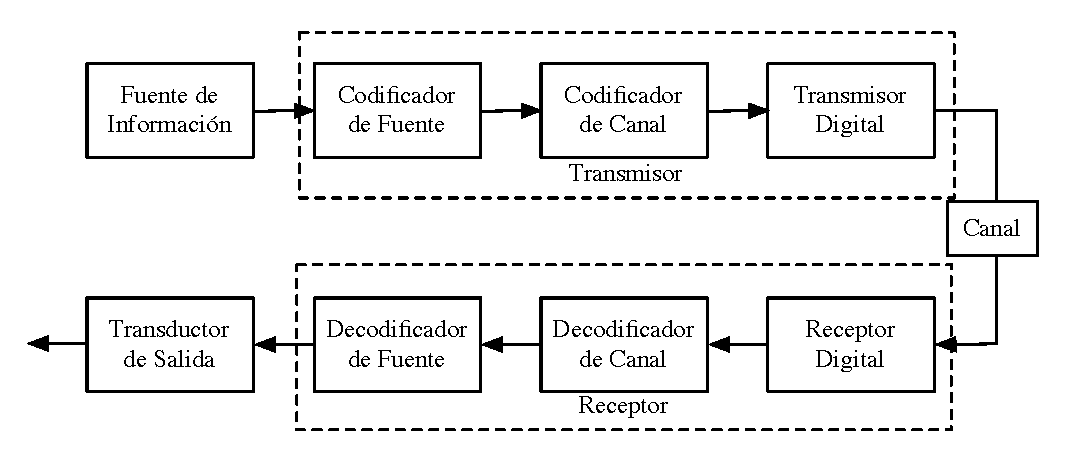
\includegraphics[width=0.95\linewidth]
{introduccion/figuras/fig01-01.pdf}
\caption{Modelo de un sistema de Comunicación Digital I}
\label{fig01-01}
\end{figure}
\end{lstlisting}
%\end{micuadro}

Y el resultado se muestra en la \autoref{fig01-01}.

%
\begin{figure}[htbp]
\centering
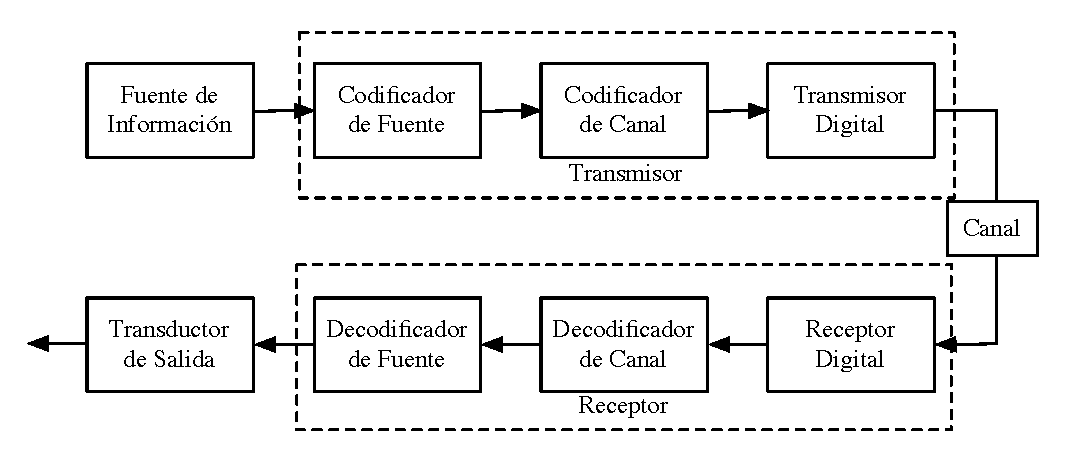
\includegraphics[width=0.95\linewidth]{introduccion/figuras/fig01-01.pdf}
\caption{Modelo de un sistema de Comunicación Digital I}
\label{fig01-01}
\end{figure}
%

Para incluir una tabla utilizamos las instrucciones siguientes:
%\nopagebreak 
\begin{lstlisting}[language=,caption={Inclusión de una tabla}, breaklines=true, label=prg01-02]
\begin{table}[htbp]
	\ttabbox
	{\caption{Tipos de transmisión y frecuencia central} 
	\label{tab2_1}}
		{
		\begin{tabular}{c c}
		\hline
		\rule[-8pt]{0pt}{22pt}{\bf Tipo de Transmisión}&
		 {\bf Frecuencia central de transmisión} \\
		\hline
		\rule{0pt}{14pt}Modem & 100-1800 Hz \\
		Radio AM & 530-1600 kHz \\
		Radio FM & 88-108 MHz \\
		Televisión & 178-216 MHz \\
		Telefonía móvil & 850 MHz-1,8 GHz \\
		Redes inalámbricas &  $2,4$ GHz \\
		Fibra óptica & $2\cdot 10^{14}$ Hz \\
		\hline
		\end{tabular}
		}
\end{table}
\end{lstlisting}

Y el resultado se muestra en la \autoref{tab2-1}.

\begin{table}[htbp]
	\ttabbox
	{\caption{Tipos de transmisión y frecuencia central} \label{tab2-1}}
		{
		\begin{tabular}{c c}
		\hline
		\rule[-8pt]{0pt}{22pt}{\bf Tipo de Transmisión}& {\bf Frecuencia central de transmisión} \\
		\hline
		\rule{0pt}{14pt}Modem & 100-1800 Hz \\
		Radio AM & 530-1600 kHz \\
		Radio FM & 88-108 MHz \\
		Televisión & 178-216 MHz \\
		Telefonía móvil & 850 MHz-$1,8$ GHz \\
		Redes inalámbricas &  $2,4$ GHz \\
		Fibra óptica & $2\cdot 10^{14}$ Hz \\
		\hline
		\end{tabular}
		}
\end{table}

Observemos  que en la parte inferior de las figuras y en la superior de las tablas (esta ha sido nuestra elección), se colocan textos explicativos sobre las mismas. El formato de este texto se logra mediante una sentencia facilitada por el paquete que se carga mediante el comando \comandos{usepackage}{caption}. El resto de paquetes utilizados realizan diversas tareas como, por ejemplo, \comandos{usepackage}{longtable}, que permite que una tabla se extienda a través de más de una página.

\subsection{Hiperenlaces}
Un primer paso a la hora de crear un documento es generar una versión en formato electrónico del mismo. Hemos decidido que ese formato sea \ttcolor{pdf} . En un formato pdf existe la posibilidad de crear hiperenlaces que facilitan la navegación a lo largo del mismo. Por ejemplo, el índice en un libro en formato pdf se generará, con la propuesta que hemos realizado, creando enlaces a las diversas partes del mismo. O bien, cuando nos referimos a una figura o tabla, es muy útil la existencia de esos enlaces al lugar exacto en el que se encuentra la figura o tabla.  El paquete responsable de realizar todas estas tareas se denomina \ttcolor{hyperref} y las sentencias que siguen a su carga realizan diversas tareas que pueden consultarse en la extensa documentación que lo acompaña. Sobre la línea 110 de \ttcolor{libroTipoETSI.tex} encontrará que puede modificar el color del enlace, puesto a negro por defecto.
% Por ejemplo, no habrá que olvidarse sustituir el literal \ttcolor{F. Javier Payán Somet y Juan José Murillo Fuentes} por el nombre del autor correspondiente.

\subsection{Tabla de contenido}
La generación de la tabla (o tablas) de contenido de un texto suficientemente largo suele ser una tarea sumamente laboriosa. \LaTeX\ facilita enormemente este trabajo mediante un conjunto de paquetes y comandos que se agrupan bajo el apartado genérico denominado TOC (Table Of Contents). En otra sección de este capítulo explicaremos cómo y dónde se incorporará esta tabla de contenidos. En este apartado nos centramos en explicar algunos aspectos de cómo se construye la principal tabla de contenidos, que denominamos  \ttcolor{Índice}.

Nuestra primera decisión fue establecer que en el índice deben aparecer hasta los apartados que hemos denominados \ttcolor{subsubsecciones}, lo que se logra mediante el \ttcolor{\{3\}} del comando \comandos{setcounter}{tocdepth} en \ttcolor{libroETSI.sty}. El formato de cada uno de los apartados se logra con el conjunto de sentencias que siguen y tienen una estructura bastante autoexplicativa. También hemos propuesto que no aparezcan los habituales puntos que existen entre el texto y el número de página correspondiente de muchos índices, ajustando a \ttcolor{10000} el parámetro \ttcolor{\textbackslash@dotsep}. 

Nuestra siguiente decisión afecta a la manera en la que hemos querido que aparezcan en el índice los índices del texto, valga la redundancia. No es trivial pero, básicamente, hemos definido dos listas, una para los elementos que aparecen antes del Índice General y otra para los  que aparecen después, al fina del texto, que se corresponden aproximadamente a lo que hemos denominado \ttcolorc{frontmatter} y \ttcolorc{backmatter}, respectivamente. Si no se desea cualquier índice, basta con comentar la línea correspondiente.

\subsection{Formatos de títulos, páginas y cabeceras y pies de páginas}
El aspecto de un libro está básicamente definido por el formato que se ha elegido para los diferentes títulos de las partes que lo constituyen, el formato de las páginas y qué queremos que aparezca en las cabeceras y pies de páginas del mismo. Todo esto se ha conseguido utilizando un paquete desarrollado por el español Bezos denominado \ttcolor{titlesec}, que se carga en nuestro fichero mediante la instrucción \comandos{usepackage[noindentafter, pagestyles,...]}{titlesec}.

El paquete nos permite definir los distintos tipos de páginas, de acuerdo con las instrucciones que se proporcionan en el mismo. Por ejemplo, con \comandos{newpagestyle}{esitscCD} creamos la página habitual en la mayor parte del texto, formada por el número en la parte exterior de la misma, en las páginas pares el nombre del capítulo en el que estamos y en las impares el nombre de la sección. Estos elementos se colocan encima de una raya horizontal que se ha definido previamente, tanto en su grosor como en su longitud.

Una vez definidos las diferentes tipos de páginas podemos definir, por ejemplo, que nuestra página por defecto será \ttcolor{esitscCD}, con la instrucción \comandos{pagestyle}{esitscCD}. Si queremos que una página determinada en un punto concreto sea diferente, si suponemos que, por ejemplo, el estilo de página \ttcolor{otroestilo} ha sido definido, basta situar la instrucción \comandos{thispagestyle}{otroestilo} en el punto deseado. Un ejemplo podemos encontrarlo en la manera que logramos que los capítulos empiecen siempre en páginas impares. Con ese fin, se utiliza el estilo de página \ttcolor{empty} en caso de que sea necesario.

Por último, el paquete \ttcolor{titlesec} nos permite definir cómo queremos que sean los titulares que usaremos en nuestros textos. Así,  la instrucción \comandos{titleformat}{\textbackslash section ...} establece que nuestras secciones estarán numeradas al nivel de capítulo, con el número de la sección fuera de margen \ttcolor{hang}, y con unas determinadas separaciones del texto, establecidas a través del comando \ttcolorc{titlespacing}. 

En todo caso, estos parámetros no se deberían de tocar, salvo en contadas ocasiones, y por ello se incluyen aquí estos detalles.

\subsection{Teoremas, propiedades, definiciones y demás}
En la escritura de cualquier texto científico los Teoremas, propiedades y demás elementos constituyen una parte muy significativa. Existen, de nuevo, múltiples posibilidades de tratar estos elementos, pero hemos considerado que las facilidades que suministra el paquete \ttcolor{ntheorem}, cargado mediante la instrucción \comandos{usepackage [thmmarks, amsmath, noconfig, hyperref, framed]}{ntheorem} se adapta perfectamente a nuestros gustos y decisiones. Por ejemplo, con el conjunto de instrucciones que se muestran en  el Código \ref{prg01-03}:

\begin{lstlisting}[language=TeX,caption={Teoremas, Lemas,...}, breaklines=true, label=prg01-03]
\theoremnumbering{arabic}
\theoremheaderfont{\aheadteoremas}
\theoremseparator{\hspace{.2em}}
\theorembodyfont{\itshape}
\newtheorem{teor}{Teorema}[section]
\newtheorem{lema}{Lema}[section]
\newtheorem{prop}{Propiedad}[section]
\newtheorem{coro}{Corolario}[teor]
\end{lstlisting}

\noindent hemos definido los Teoremas, Lemas, Propiedades y Corolarios. Centrándonos en los teoremas, las instrucciones anteriores definen que los teoremas estarán referenciados mediante un número \ttcolor{arabic}, con una numeración que será creciente desde la unidad dentro de cada sección de un determinado capítulo, \comandos{newtheorem\{teor\}}{Teorema}\ttcolor{[section]}. La fuente que se utilizará para que aparezca la palabra ``Teorema'' está definida por el comando \ttcolor{\textbackslash theoremheaderfont\{\textbackslash aheadteoremas\}}, el enunciado del teorema se realizará en itálica y para enunciar un teorema y su demostración utilizamos las siguiente instrucciones:

\begin{lstlisting}[language=TeX,caption={Teorema y Demostración}, breaklines=true, label=prg01-04]
\begin{teor}[Teorema de Pitágoras]
En un triángulo rectángulo...
\end{teor}
\begin{proof}
Sea el triángulo ABC...
\end{proof}
\end{lstlisting}

El resultado sería el siguiente:
\begin{teor}[Teorema de Pitágoras]
En un triángulo rectángulo...
\end{teor}
\begin{proof}
Sea el triángulo ABC...
\end{proof}

Podemos observar que al finalizar la demostración hemos incluido el símbolo $\blacksquare$. De manera análoga, están definidas las restantes entidades, incluyendo el comando que nos permite escribir los cuadros de elementos de la programación.

\subsection{Índices de palabras y glosarios}
Con los paquetes index y glossaries podemos incluir índices de palabras y listas con definiciones, ya sea de acrónimos u de otro tipo. Por ejemplo, se podría usar también para definir magnitudes o la notación utilizada.
 
%http://en.wikibooks.org/wiki/LaTeX/Indexing
\subsubsection{Índices de palabras}
\index{Indice de palabras@Índice de palabras!index}%\index{\'Indice de palabras!index}\index{Índice de palabras!indexit}
Para construir un índice de palabras\index{Indice de palabras@Índice de palabras}, como el que puede encontrar al final de este texto, se incluye el paquete \comandos{usepackage}{imakeidx} con algunas opciones. Para incluir una palabra  en el índice utilizamos   \comandos{index}{palabra} justo detrás de la palabra que queramos indexar. Si queremos agrupar en un grupo diferentes subpalabras \index{Indice de palabras@Índice de palabras!subpalabra}, utilizamos \comandos{index}{palabra!subpalabra}. Es importante no olvidar ejecutar \ttcolor{makeindex}, al igual que ejecuta latex o bibtex para componer el texto o generar la bibliografía. Otro detalle importante es poner los índices con mayúsculas o con minúsculas, pero todos iguales. De esta forma, cuando se genere el índice de palabras no queden algunas con la primera letra en mayúsculas y otras no. Por último, con las instrucciones de compilación que se detallan un poco más adelante, las palabras en español que empiecen por tilde se indexan al final. Para evitarlo, y que aparezcan en su sitio, tiene que escribir primero la palabra sin tilde seguida de arroba y la palabra con tilde, como por ejemplo \ttcolorc{index\{Indice de palabras@Índice de palabras\}}. 

\subsubsection{Glosario}
Un glosario con acrónimos u otros términos se realiza en este texto utilizando\\
 \comandos{usepackage [acronym]}{ glossaries}. 
 Para definir un acrónimo, basta con incluir antes del comienzo del documento una línea del tipo:\\
 \comandos{newacronym[type=main]\{etiqueta\}\{acrónimo\}}{nombre completo}, 
 \\
 como por ejemplo\\
 \comandos{newacronym[type=main]\{ETSI\}\{ETSI\}}{Escuela Técnica Superior de \\Ingeniería}. 
 \\
 En esta orden el primer argumento es el identificador o etiqueta, el segundo es el acrónimo o abreviatura y el tercero es el nombre completo al que hace referencia el acrónimo o abreviatura. Para utilizar luego la abreviatura o acrónimo, y se pueda luego generar un índice que indique en qué página se ha usado, se utiliza \comandos{gls}{etiqueta}. 

\subsubsection{Compilación de índices de palabras y glosarios}
Existen distintos comandos para generar el índice y el glosario. Puede utilizar los que estime oportunos. Aquí se ofrece una solución para realizarlo.

El comando más usado es \ttcolor{makeindex}. Habría que llamar dos veces a este comando, con distintos argumentos, si se incluye el glosario además del índice. En Macintosh si utiliza el comando \ttcolor{lualatexmk}, uno de los engines de TeXShop\index{engine}, el índice de palabra y el glosario se generarán de forma automática. 
%Puede usar Texindy\index{Texindy} para una presentación del índice de palabras con otra presentación.

En Windows, tendrá que ejecutar PDFLatTeX ó LatexMk, luego tendrá que ejecutar makeindex tal cual para generar el índice de palabras. Para generar el glosario tendrá que definir un comando de usuario, tal como sigue. Vaya al menú `Usuario', en texmaker, y allí a `Comandos de Usuario' y dentro de este a `Editar Comandos de Usuario'. En cualquiera de los comandos defina uno nuevo con el título que quiera, por ejemplo glosario, y en el campo comando, incluya la siguiente línea\footnote{Si usase el texmaker en Mac-OS tendría que pulsar el asistente para seleccionar makeindex. Aparecería en el campo comando algo así como \ttcolor{''makeindex'' \%.idx}, donde el asistente habrá encontrado la carpeta donde está el comando makeindex. Sustituya el final, \%idx, por  -s \%.ist -t \%.glg -o \%.gls \%.glo, de forma que el campo comando quede como sigue:
 \ttcolor{''/usr/texbin/makeindex'' -s \%.ist -t \%.glg -o \%.gls \%.glo}}

Una vez definido este comando de usuario, ejecútelo, y vuelva a ejecutar PDFLaTeX o LatexMk.

\section{Antes del documento}
Antes de empezar la edición del documento, además de cargar los ficheros de estilos \ttcolor{LibroETSI.sty} y \ttcolor{edicionLibro.sty} (o el correspondiente al documento),  hemos creído necesario realizar una serie de operaciones que faciliten nuestro trabajo o lo configuren de una determinada manera. %Además, hay que incluir la portada.

\subsection{Fichero de notación: notacion.sty}
Hemos considerado interesante incluir un fichero de notaciones que son de amplia utilidad dentro del área de conocimiento de los autores. Su uso es completamente opcional pero se ha utilizado ampliamente en la elaboración de este texto. Simplifica enormemente la escritura hacer uso de ficheros de este tipo y prácticamente cada autor utiliza el suyo propio.

Como ocurría con el fichero \ttcolor{LibroETSI.sty}, es necesario que se cargue, incluyendo la instrucción \comandos{usepackage}{notacion} al comienzo del fichero principal. Puesto que su uso resulta evidente, no hemos considerado necesario realizar una documentación precisa sobre el mismo más allá de los propios comentarios que acompañan las definiciones del fichero, y que el lector puede consultar abriéndolo. Nótese que existe además una carpeta con este nombre. En esta carpeta se ha incluido un ejemplo de notación que podría ponerse al comienzo de un documento. Sobre este documento, se puede añadir o quitar lo que se desee.

\subsection{Fuente del texto}
Las instrucciones incluidas en el código \ref{prg01-05} y que pertenecen al fichero \ttcolor{LibroETSI.sty} 
 se pueden modificar para cambiar la fuente del texto.  En primer lugar, debemos actuar de forma diferente si queremos utilizar la fuente Minion Pro o no.  Si hemos definido como \ttcolor{true} el parámetro correspondiente, en el caso que estemos compilando con \LaTeX\ no debemos hacer nada. Sin embargo, en el caso de utilizar \LuaLaTeX\ debemos declarar que la fuente va a ser Minion Pro y modificar ligeramente su tamaño.
 
Si no vamos a utilizar una fuente Minion Pro, en el caso de \LuaLaTeX\ se puede utilizar para el texto cualquier fuente OTF o TTF que el usuario posea de forma legal, y se encuentre instalada, lo que depende del sistema operativo (SO) utilizado. En nuestro caso, observad que hemos utilizado una fuente Time New Roman  pues suele estar instalada en la mayoría de los SO. Se proponen asimismo un par de alternativas si prefiere otras fuentes.
 
El código incluido detecta si se no se está utilizando \LuaLaTeX\, en cuyo caso se usa una fuente equivalente a una Times, cargada mediante el comando estándar \comandos{usepackage}{tgtermes}. Hay otras opciones comentadas, y se pueden buscar otras fuentes. 
 
\begin{lstlisting}[language=,caption={Fuente del texto}, breaklines=true, label=prg01-05]
%:Para modificar fácilmente la fuente del texto. 
\makeatletter
\ifdtsc@Minion % Queremos utilizar la fuente Minion y lo hemos declarado al principio
	\ifluatex
		\setmainfont[Renderer=Basic, Ligatures=TeX,	% Fuente del texto 
		Scale=1.01,
		]{Minion Pro}
   		% En este caso conviene modificar ligeramente el tamaño de las fuentes matemáticas
		\DeclareMathSizes{10}{10.5}{7.35}{5.25}
		\DeclareMathSizes{10.95}{11.55}{8.08}{5.77}
		\DeclareMathSizes{12}{12.6}{8.82}{6.3}
	\fi
\else
	\ifluatex
		% Para utilizar la fuente Times New Roman, o alguna otra que se tenga instalada
		\setmainfont[Renderer=Basic, Ligatures=TeX,	% Fuente del texto 
		Scale=1.0,
		]{Times New Roman}
%		\setmainfont[Renderer=Basic, Ligatures=TeX,	% Fuente del texto 
%		]{Adobe Garamond Pro}
%		\setmainfont[Renderer=Basic, Ligatures=TeX,	% Fuente del texto 
%		]{Palatino LT Std}
	\else
		\usepackage{tgtermes} 	%clone of Times
		%\usepackage[default]{droidserif}
		%\usepackage{anttor} 	
	\fi
\fi
\makeatother
\end{lstlisting}

Si se intenta utilizar una fuente que no está instalada (dentro del sistema operativo) la compilación con \LuaLaTeX\ daría error. Si se instala una nueva fuente y se desea utilizar, se puede tratar de modificar las líneas de código que se suministran como ejemplo. La primera vez que se utilice esa nueva fuente, \LuaLaTeX\ tardará algo más en compilar pues necesita generar una serie de ficheros internos.

La principal ventaja en el uso de \LuaLaTeX\ la encontramos en la facilidad para utilizar diferentes fuentes en diferentes lugares y con diferentes características (tamaño, color, etc) muy fácilmente configurables. Puede ser interesante leer el fichero \ttcolor{fontspec.pdf} para conocer cómo se realizan estos cambios. 

En caso de utilizar el motor pdfLatex, la elección más sencilla se realiza como hemos dicho mediante paquetes específicos tales como \comandos{usepackage}{tgtermes}. Puede consultarse la dirección \url{http://www.tug.dk/FontCatalogue/alphfonts.html} para conocer las posibilidades más habituales. 

Por último: como ya hemos dicho, todo lo anterior únicamente afecta a la elección de las fuentes del texto. La elección de las fuentes matemáticas (texto dentro de matemática, símbolos, letras griegas, etc) se controla de manera completamente diferente mediante paquetes específicos. En el \autoref{estilo} volveremos sobre este asunto. En concreto, observar que en el caso de compilar con la opción \ttcolor{Minion=true} y existir el fichero de estilo \ttcolor{MinionPro.sty} (no confundir con la fuente Minion Pro; si no existiera el fichero, aparecería un error), se propone el uso de la fuente Minion Pro como fuente matemática, junto con los símbolos de la fuente MnSymbol. En caso contrario, se hará uso de una fuente Times (en realidad, de una extensión de la misma). 

No todas las fuentes pueden usarse como fuentes matemáticas y en la dirección \url{http://www.tug.dk/FontCatalogue/alphfonts.html} se encuentran recogidas las que si tienen soporte matemático. Es importante señalar además que no todas las combinaciones de fuente de texto y fuente matemática son tipográficamente adecuadas. 

\subsection{Cubierta y primeras páginas}
Se ha diseñado esta plantilla para que tome una imagen de fondo y a partir de ésta se incluyan los datos de título, autor, etc, para generar la portada del documento. La portada propuesta es distinta para proyectos fin de carrera y similares que para libros o tesis. Todo esto se ha hecho diseñando una serie de funciones que las generan, tomando los datos que se definen en la cabecera del fichero principal. Así, en el \ttcolor{libroTipoETSI.tex}, se puede definir el título de la obra, el autor, etc. En el caso de \ttcolor{pfcTipoETSI.tex} y \ttcolor{tesisTipoETSI.tex}, se puede definir además el director, el tipo de proyecto (máster, grado y carrera), y otros parámetros. Las imágenes de fondo de la cubierta también se llaman desde este fichero, así como la imagen al pié de la hoja interior con el título y autor de la obra (para libros). La imagen central de la cubierta está en la carpeta figuras, con nombre \ttcolor{imagenLibro.png}. Puede incluir la imagen deseada en esta carpeta salvándola con este mismo nombre. Preste atención a que el formato es rectangular. Para introducir la imagen del logo del departamento en el proyecto fin de carrera/grado/máster, puede retocar la imagen de fondo, cortando el logo existente e insertando el deseado. Estas imágenes están en la carpeta figuras. 

Para cambiar cualquier otro aspecto, tales como el tamaño de la figura de la cubierta ó los créditos de la cubierta, tendrá que modificar el fichero \ttcolor{edicionLibro.sty} en este caso de un libro. 

%En el ejemplo que se presenta para libros, el latex toma una imagen de fondo, y otra, imagenLibro.png,  de la portada para incluir además de los datos de título y autores, definidos al comienzo del fichero \ttcolor{portadaLibro.tex}, una imagen superpuesta representativa de la temática del texto. Los autores pueden cambiar esta imagen fácilmente por otra acorde a su texto.

%Sería interesante poner algo sobre citas

\endinput

%
% !TEX root =../LibroTipoETSI.tex
\chapter{Denegación de Servicio}\LABCHAP{Denegacion de Servicio}
\pagestyle{esitscCD}
\epigraph{ Denial of Service: ``The prevention of authorized access to resources or the delaying of time critical 
operations''. }{ITU-T recommendation X.800}

% TODO terminar introducción del capítulo
% TODO cambiar todos los TCP, UDP, ICMP, SYN, ACK, DNS por sus acrónimos
%\lettrine[lraise=0.7, lines=1, loversize=-0.25]{E}{l} 
\lettrine[lraise=-0.1, lines=2, loversize=0.25]{E}n este capítulo trataremos de definir qué es un \gls{DoS} 
\index{DoS}, qué significa que un ataque de denegación de servicio sea distribuido \acrshort{DDoS} \index{DDoS}, por 
qué es importante su prevención, por qué es tan difícil su identificación y defensa, esto es, la motivación del 
proyecto.

Las diferentes secciones seguirán la misma clasificación que siguen S.V. Raghavan y E. Dawson en su libro ``An 
Investigation into the Detection and Mitigation of Denial of Service (DoS) Attacks'' \cite{Raghavan}.

%http://en.wikibooks.org/wiki/LaTeX/List_Structures#Customizing_Lists
\section{Definición y consecuencias de un ataque de denegación de servicio} \label{sec:Tipos de ataques DoS}
La seguridad de la información se puede dividir en tres sectores: confidencialidad, esto es, la 
información sólo es vista por los destinatarios; integridad, esto es, la información no ha sido 
alterada desde que se registró y, por último, disponibilidad: El destinatario puede obtener la 
información siempre que la necesite. Un sistema es seguro en la medida que cumple estas tres 
condiciones.

La definición formal que ofrece la \gls{ITU-T} en su recomendación X.800 es la siguiente \cite{ITU-T_DDoS_def}:

\begin{quote}
 The prevention of authorized access to resources or the delaying of time critical operations.
\end{quote}

Por su parte, el \gls{CNSS} ofrece una definición más general \cite{CCNS_DDoS_def}:

\begin{quote}
 Any action or series of actions that prevents any part of an information system from functioning.
\end{quote}

Así pues, los ataques de denegación de servicio atacan directamente a la disponibilidad. Esta falta de disponibilidad 
pueda ser debida a acciones maliciosas o no, originadas de manera local al sistema que se desea proteger o remotamente.

Para impedir el acceso a los recursos, el atacante puede atacar cualquier eslabón de la cadena: Desde el ancho de banda 
de la red que conecta el usuario con el mismo, la memoria o capacidad de procesamiento de la que dispone el sistema, 
alguna debilidad del protocolo de red o la aplicación usada, o cualquier otro sistema que consiga dicho fin 
\cite{Raghavan}.

De esa forma, la empresa que posee el recurso se queda sin los beneficios que el mismo genera durante un periodo de 
tiempo. 

\section{Divide y vencerás: DoS distribuidos}
La principal clasificación que se puede hacer de los ataques de denegación de servicio es en base al número de 
ordenadores atacantes. Si hay más de uno, entonces estamos hablando de un ataque de denegación de servicio distribuido. 
No se debe confundir con los tipos \emph{Spoofing}\footnote{Se definirán mejor estos ataques en el 
\SSSEC{DoS por inundacion}}, que consisten realmente en falsear la dirección de origen de 
las PDU usadas en el ataque. Tras ello, todos los ataques que describiremos a continuación pueden ser distribuidos o no 
(aunque, obviamente, los ataques relacionados con la fuerza bruta tienen más sentido distribuirlos que aquellos que no).

No es raro ver que los atacantes son cientos o miles, y se han llegado a registrar ataques con millones de atacantes. 
La mayoría de los atacante son simplemente nodos infectados con algún tipo de virus o gusano informático, controlados 
y sincronizados remotamente. Estos ordenadores, entonces, pasan a denominarse ordenadores zombis o \emph{bots} 
\index{Bot} \index{Zombi}, controlados por un nodo maestro, y pasan a formar parte de la llamada 
\emph{botnet}\index{Botnet}. Este tipo de ataques se describirán también, más detalladamente, en el \SSSEC{DoS por 
inundacion}.

\section{Taxonomía de un ataque de denegación de servicio}
Las definiciones dadas hasta ahora de ataque de denegación de servicio han sido bastante amplias: Hemos acotado qué 
queremos defender, pero no cómo pueden atacarlo, ni qué parte del sistema de comunicación atacarán. Y esto es necesario 
si queremos definir un sistema de defensa efectivo.

A modo de simplificación, en este trabajo asignaremos a los ataques de denegación de servicio dos características 
diferenciadoras: Sistema de ataque, y objetivo del ataque. De esta forma, podremos entender el por qué del diseño del 
sistema de defensa escogido.

\subsection{Sistema de ataque}
\subsubsection{DoS por inundación}\LABSSSEC{DoS por inundacion}\index{Ataques por inundación} \index{Flooding attacks}
Bajo esta categoría clasificaremos aquellos ataques dirigidos a agotar los recursos que realizan alguna función 
directamente relacionada con ofrecer el servicio. Principalmente, los recursos objetivos suelen ser la memoria, la CPU 
y el ancho de banda, aunque también pueden ir dirigidos a agotar, por ejemplo, el espacio de almacenamiento disponible. 
De esa forma, no queda ningún recurso para que un usuario legítimo pueda hacer uso de ellos.

Este tipo de ataque necesita que el atacante tenga suficientes recursos como para limitar los del atacado. Normalmente, 
un solo atacante no tendrá recursos suficientes para saturar, por ejemplo, un servicio expuesto a Internet. Es ahí 
donde resalta la utilidad de usar un ataque distribuido: Muchísimos atacantes pequeños son capaces de tumbar un 
servicio preparado para atender muchos clientes.

Actualmente, se ofrecen en Internet muchísimos servicios de botnets, haciendo que llevar a cabo un ataque de fuerza 
bruta por inundación sea fácilmente realizable.

Un ejemplo clásico de este tipo de ataque es la inundación de paquetes SYN\index{SYN} TCP\index{TCP}. Para que una 
conexión TCP llegue a ser válida, es necesario que el cliente envíe al servidor \index{Servidor} un paquete TCP de 
sincronía (esto es, con la bandera SYN activa), el servidor le responda con un paquete SYN+ACK \index{ACK} (esto es, con 
las dos banderas activas, SYN y ACK) y el cliente \index{Cliente} devuelva un primer ACK.

Si un cliente sólo envía paquetes SYN, el servidor se ve obligado a mantener una serie de conexiones medio abiertas, lo 
cual terminará por agotar los recursos del servidor (la víctima).

\paragraph{Ataques coordinados por seres humanos}\mbox{\newline}

\noindent Si existen muchos atacantes que requieren intervención manual para realizar el ataque, estamos hablando de un 
ataque DDoS coordinado por seres humanos. 

Un ejemplo de este tipo de ataque es el ataque denominado F5 \cite{F5_attack}. En él, un estudiante intentó tirar abajo 
la red de su escuela convenciendo a muchos estudiantes de que se conectasen a una página determinada y, a una hora 
concreta, presionasen al mismo tiempo el botón \emph{F5} (actualizar página en la mayoría de los navegadores) durante 
un periodo de tiempo.

Otro ejemplo de ataques de este tipo suceden con bastante frecuencia en el denominado \emph{efecto slashdot} (o, el 
equivalente español, efecto barrapunto/menéame). Slashdot es un servicio de noticias muy usado en todo el mundo, al 
igual que sus equivalentes españoles meneame y barrapunto, en el que se acumulan enlaces a noticias subidas por los 
propios usuarios, que son votadas y promocionadas.

Cuando una de esas noticias se encuentra alojada en un servidor con pocos recursos, es frecuente que esta quede 
inaccesible por sobrecarga de recursos. Pese a que la intención de los usuarios era legítima, el sitio ha sufrido un 
\gls{DDoS} según las definiciones anteriores.

\paragraph{Ataques amplificados}\mbox{\newline} \index{Ataques amplificados}

\noindent Un ataque amplificado ocurre cuando el atacante es capaz de generar una respuesta automática de muchos nodos 
de la red, dirigidas a la dirección de la víctima. En la \FIG{amplificacion} podemos ver una descripción gráfica de lo 
que ocurre en este ataque.

\begin{figure}[htbp]
\centering
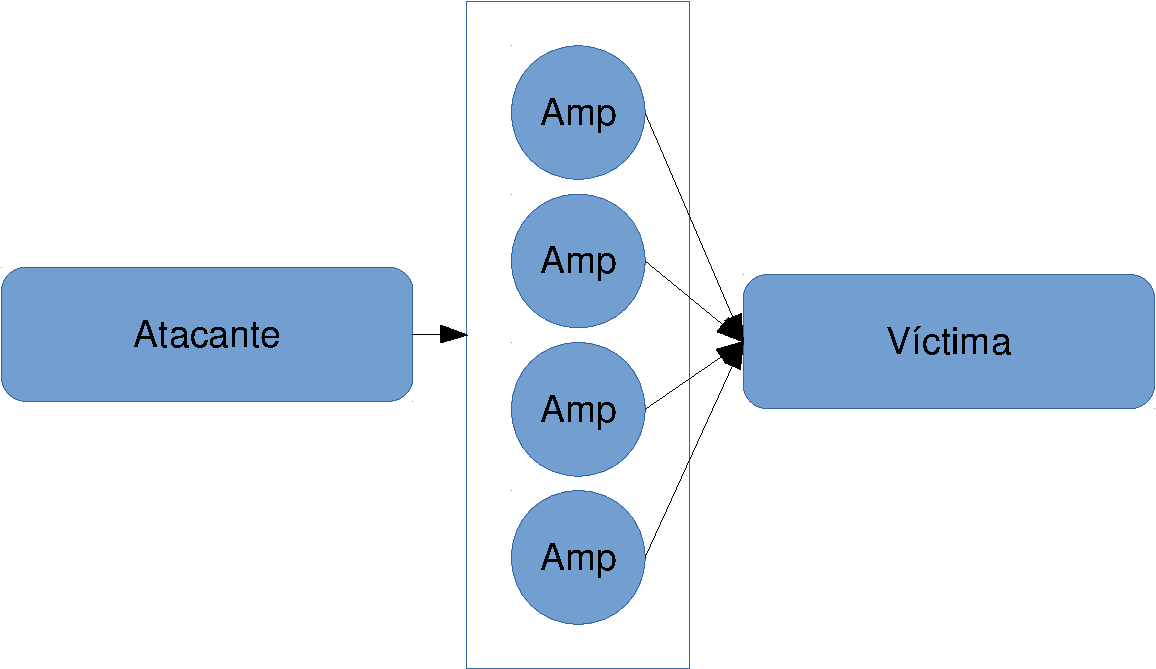
\includegraphics[width=.8\textwidth]{CapituloDDoS/Figuras/Amplificacion}
\caption{Ataque por amplificación}
\LABFIG{amplificacion} %Esto es una forma propia de los autores de gestionar las etiquetas y referencias
\end{figure}
%

Normalmente, este tipo de ataques utilizan la dirección de difusión o broadcast \index{Broadcast} \index{Difusión}. La 
dirección de difusión es una dirección especial en las redes en las que todos los nodos recibirán el paquete. Si ese 
paquete es una petición que requiere una respuesta, y tiene como dirección origen la dirección IP de la víctima (IP 
spoofing\index{IP Spoofing}), todos los nodos de la red responderán el mensaje, saturando la máquina objetivo.

Un ejemplo sencillo de este tipo de ataque es el denominado Ataque \emph{Smurf} \index{Smurf}, que utiliza un 
simple ICMP\index{ICMP} PING\index{ICMP}\index{PING}. Si a todos los nodos de la red les llega una petición de PING 
proveniente de la dirección de la víctima, la víctima se encontrará con tantas respuestas como nodos configurados para 
responder tenga la red. Dichas respuestas tendrán que ser, al menos, procesadas por el sistema operativo de la máquina 
objetivo, que terminará saturando. Por otro lado, el contenido de la respuesta será una copia del contenido de la 
petición, por lo que es sencillo multiplicar (amplificar) el ancho de banda consumido por la víctima emitiendo un 
paquete grande.

Una variante del anterior es el ataque \emph{Fraggle}. El protocolo UDP\index{UDP} tiene su propio sistema de PING, en 
el puerto 7. Además, tiene un sistema de generación de cadenas aleatorias en el puerto 19, el cual envía cadenas de 
texto aleatorias de longitud aleatoria (pero reducida) cualquiera que las pida. De nuevo, la mecánica del ataque es 
falsear la dirección de origen para que estos servicios respondan a la víctima, saturando así la capacidad de sus 
recursos.

\paragraph{Ataques reflejados}\mbox{\newline} \index{Ataques reflejados}

\noindent Para este apartado, un reflector es un nodo que responde a un paquete con otro paquete destinado a la 
dirección origen del primer paquete. Así, podríamos englobar en este apartado, por ejemplo, servidores DNS\index{DNS}. 
Ver \FIG{reflexion}.

\begin{figure}[htbp]
\centering
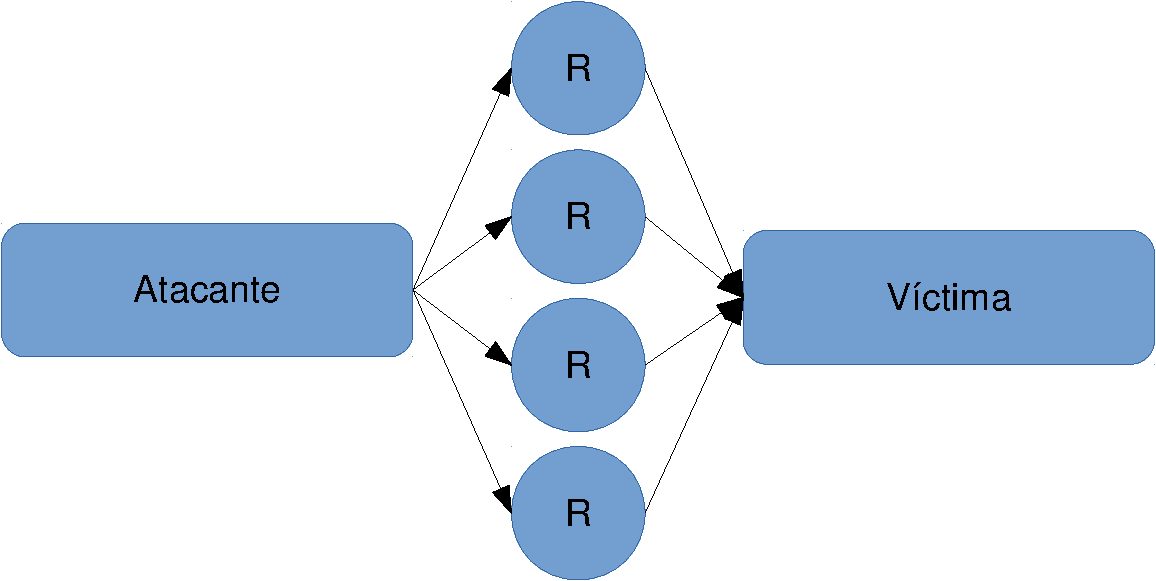
\includegraphics[width=.8\textwidth]{CapituloDDoS/Figuras/Reflexion}
\caption{Ataque por reflexión}
\LABFIG{reflexion} %Esto es una forma propia de los autores de gestionar las etiquetas y referencias
\end{figure}
%

El atacante, entonces, crea una lista de IP reflectoras, y envía para el ataque una petición a cada una de las 
direccionas, con dirección origen la de la vícima. De esta forma, localizar y detener el ataque se vuelve mucho más 
difícil, ya que, siguiendo el ejemplo, cada servidor DNS tiene un dirección IP que no tiene nada que ver con el resto.

Sin embargo, nada impide, en principio, combinar este ataque con el tipo amplificación (por ejemplo, si se 
disponen de muchos DNS en la misma subred). Por otra parte, es posible hacer una petición recursiva a un servidor DNS, 
de forma que en la respuesta viaja el resultado de cada servidor DNS. Esto es, con una pequeña petición (cabecera UDP, 
DNS y nombre de dominio pedido) obtenemos una respuesta mucho mayor, y ya dirigida a la dirección de la victima. 

Así pues, la diferencia entre este tipo y el anterior es que el atacante necesita de una lista de direcciones de host, 
e ir iterando para conseguir el efecto deseado, mientras que en la otra cada paquete se amplificaba mediante el uso de 
la difusión.

\paragraph{Ataques basados en botnets}\mbox{\newline}

\noindent Un bot o zombi es un equipo infectado y controlado remotamente por un maestro. Éste puede ser usado para 
enviar correo no deseado, distribuir malware, espiar (esnifar\index{Esnifar tráfico}) tráfico o, en nuestro caso de 
estudio, para perpetrar un ataque de denegación de servicio. 

Gracias a la red de zombis, el atacante real es mucho más difícil de localizar, además de servir como una primera etapa 
de amplificación del ataque.

\subsubsection{DoS Semánticos}\LABSSSEC{DDoS semanticos}
Esta segunda forma de ataque no se basa en la fuerza bruta o en la extenuación de recursos, sino en 
provocar que el servidor\footnote{O algún elemento de la infraestructura de la comunicación} entre en un estado 
\emph{ilegal}, de forma que no pueda ofrecer el servicio. No es necesario un atacante (o varios) con mucha fuerza, sino 
que se puede llevar a cabo con muy pocos recursos. Sin embargo, requiere un conocimiento mucho más profundo del 
servidor y canal de comunicación. Eso sí, el ataque es más sutil y, lo más importante, puede ser corregido con una 
adecuada configuración o actualización de componentes.
 
Uno de los principales ataques de este estilo consiste en enviar información concreta que sabemos de antemano que 
provocará una caída o malfuncionamiento en el servidor, es decir, aprovechando un fallo de seguridad. Por ejemplo, hasta 
hace relativamente poco (1997), el famoso \emph{ping de la muerte}\index{Ping de la Muerte} \cite{Bidou} era capaz de 
tumbar un servidor con tan 
sólo un comando: \texttt{ping <objetivo>\ -l 65511}, el cual viene integrado en todos los sistemas operativos. Éste 
aprovechaba que la pila ICMP asumía que el paquete tenía una longitud determinada. Al procesar el paquete, y superarse 
esta longitud, se producía un desbordamiento de buffer que hacía que el servidor colapsase.

Otro ejemplo de ataque de este tipo es el ataque \emph{land\index{Land attack}}. En él, la victima recibe un paquete 
TCP cuya dirección origen y destino es él mismo, por lo que intenta contactar consigo mismo hasta que colapsa. 

El ataque \emph{\index{Teardrop}} también es muy famoso, consistente en enviar mensajes IP fragmentados y malformados a 
la muina objetivo. De esta forma, al intentar des-fragmentarlos, la máquina colapsa.

Las nuevas tecnologías tampoco son inmunes a este tipo de ataque. IPv6, por ejemplo, puede sufrir de \emph{Anuncio de 
vecino envenenado\index{Neighbour Advertisement Spoofing Attack}}. En él, un equipo intermedio se anuncia como poseedor 
de una dirección en el camino del cliente al servidor (o bien, la dirección del propio servidor), y anuncia su 
dirección MAC para que todos los paquetes destinados al servidor le lleguen a él. Esto es, es la versión IPv6 del ARP 
spoofing.

\subsection{Objetivo del ataque}
Si queremos ser capaces de defendernos ante un ataque DDoS, es necesario conocer a qué objetivos van destinados. De esa 
forma, podremos centrarnos en defender los activos vulnerables de una forma eficiente.

Podemos clasificar los ataques según el nivel de la capa OSI que atacan en ataques a los routers, a la red, al SSOO o a 
la propia aplicación. Obviamente, un ataque a un nivel inferior afectará a todos los niveles superiores.

\subsubsection{Ataque a dirigido a redes}
La red es el componente más básicos de los ataques DDoS. Si el cliente es incapaz de conectar con la red del servicio, 
es imposible que éste pueda ser ofrecido. Por su parte, si la red del servicio está saturada, ningún cliente será capaz 
de acceder a la misma.

Para agravar las cosas, las aplicaciones confían cada vez más en servicios dependientes de la red. Ejemplo de ello es 
la proliferación de servicios web\index{Servicio web} (aquellos que usan el protocolo \acrshort{HTTP} para su 
funcionamiento), o los servicios en la nube\index{Servicio en la nube} (esto es, aquellos en los que el almacenamiento 
y procesado de datos se realiza en ordenadores remotos, a los que se accede por Internet). 

No solo las redes corporativas exponen sus servicios a Internet. Poco a poco, sistemas críticos, tales como plantas 
generadoras de energía o de procesado de agua, están dentro de una red que, a su vez, en unos pocos saltos están 
conectadas a Internet. De esta forma, estos servicios podrían ser víctimas de un ataque DDoS. Es posible, incluso, que 
el lanzar un ataque hacia otro servicio en esta red intermedia afecte a dicho servicio crítico \cite{Raghavan}.

Así pues, un ataque de denegación de servicio que afectase a dicha infraestructura crítica podría tener repercusiones 
muy serias, tales como dejar sin energía o agua una zona del mapa, y que pocos sistemas escapan actualmente de la 
posibilidad de un ataque DDoS: En el momento que lo conectas a Internet, estás expuesto a ello.

Uno de los protocolos más usados para el transporte de información es \gls{TCP}, por lo que un gran porcentaje de 
ataques van dirigidos contra esta tecnología.

\paragraph{Reseteo de conexiones}\mbox{\newline}

Un ataque muy simple consiste en, una vez que el atacante conoce una conexión existente, resetear dicha conexión. Una 
conexión en \gls{TCP} está identificada por una dirección origen, una dirección destino, un puerto origen y un puerto 
destino. Existe un bit RST\index{TCP RST} en la cabecera \gls{TCP} que permite resetear una conexión inmediatamente. 
Esto es usado, por ejemplo, si uno de los dos extremos detecta un problema en la conexión. Para terminar de empeorar 
las cosas, RST no necesita ACK, por lo que el cliente no llega a saber que la conexión ha terminado

Tras recibir el servidor el RST, el cliente continúa enviando paquetes, y se encontrará con un socket cerrado. El 
servidor enviará otro RST, y será imposible mantener la conexión durante un largo periodo de tiempo. 

Si el atacante ha conseguido localizar una conexión, y es capaz de enviar un paquete TCP con dicho bit activo, el 
receptor de dicho paquete no aceptará más paquetes de esa conexión, y, por tanto, se habrá conseguido que la conexión 
quede invalidada. Podemos ver una descripción gráfica de este ataque en la \FIG{RST attack}.

\begin{figure}[htbp]
\centering
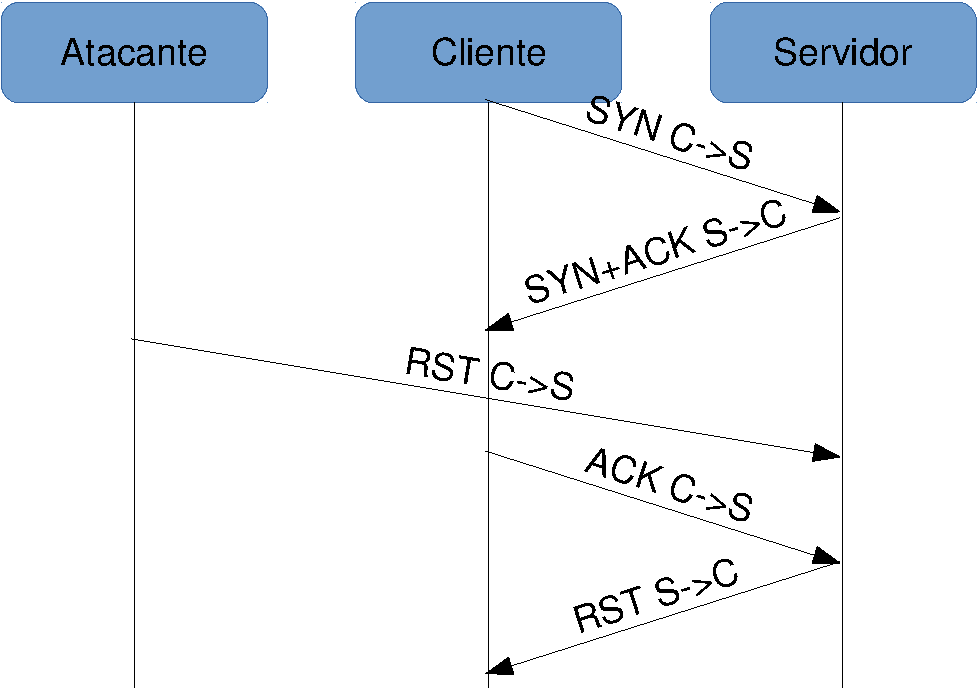
\includegraphics[width=.8\textwidth]{CapituloDDoS/Figuras/RST_attack}
\caption{Ataque RST}
\LABFIG{RST attack} 
\end{figure}
%

\paragraph{Asentimientos optimistas}\mbox{\newline}

Otra característica comúnmente explotada de las conexiones \gls{TCP} es su control de congestión\index{Control de 
congestión TCP}. Para calcular la saturación del enlace, un extremo considera como paquete perdido (y, por tanto, el 
enlace está saturado) aquel paquete que tarda más de $T$ segundos en recibir el ACK. Al iniciar la conexión TCP, el 
algoritmo de arranque lento\index{TCP slow start} incrementará el número de paquetes enviados de una forma exponencial.

Si el atacante envía ACK optimistas, esto es, ACK de un paquete que realmente no ha recibido aún, el atacante enviará 
cada vez más y más paquetes salientes, hasta saturar su conexión. Teniendo en cuenta que un TCP ACK sólo ocupa 54 
bytes, el efecto amplificador de este tipo de ataque es bastante importante. Algunos estudios hablan de que, con una 
conexión de 56kbps, es posible generar en el lado del atacante unos 8.9mbps \cite{sherwood}.

Podemos ver un ejemplo de este tipo de ataques en la \FIG{optim ACK attack}.

\begin{figure}[htbp]
\centering
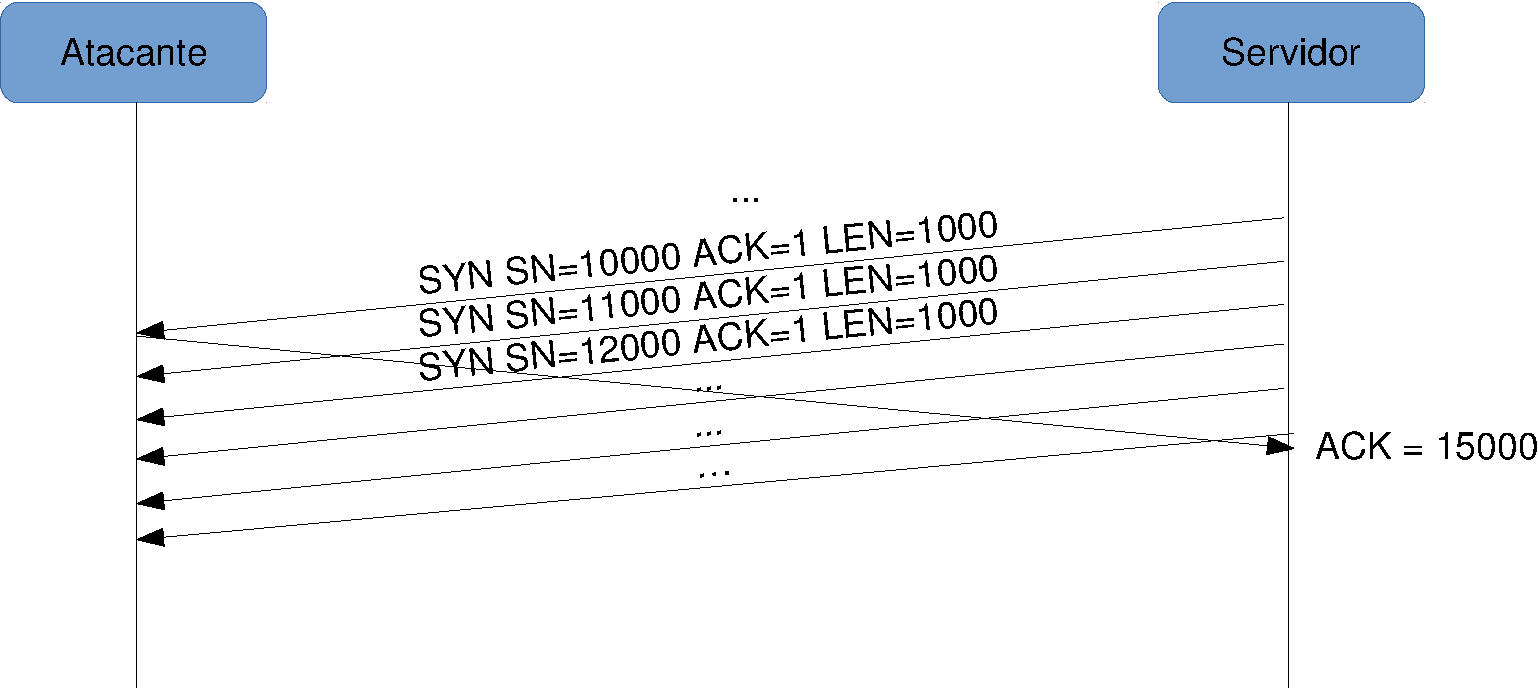
\includegraphics[width=\textwidth]{CapituloDDoS/Figuras/optim_ACK_attack}
\caption{Ataque por ACK optimista}
\LABFIG{optim ACK attack} 
\end{figure}
%

\paragraph{Temporizador de retransmisión}\mbox{\newline}

Cuando un paquete se pierde en una conexión \gls{TCP}, el protocolo dice que es necesario reenviarlo. Como ya hemos 
explicado, un paquete perdido es aquel que no recibe el ACK correspondiente.

El atacante podría saturar los dispositivos de comunicación si envía una gran inundación de paquetes a los mismos. Sin 
embargo, esto sería fácilmente detectable por dispositivos que monitorizan la red.

En su lugar, el atacante enviará una ráfaga de corta duración pero de mucha intensidad, lo suficiente para saturar los 
dispositivos y hacer perder paquetes. En este caso, \gls{TCP} alcanzará el estado de \emph{timeout} en todas las 
comunicaciones, y necesitará comenzar a retransmitir los paquetes por donde iba la conexión.

Siguiendo el procedimiento de \gls{TCP}, se debe comenzar a retransmitir los paquetes en ráfagas, empezando por un 
paquete por ráfaga e ir aumentando progresivamente. En poco tiempo, se debería volver a alcanzar un buen rutmo para la 
conexión.

Sin embargo, si el atacante, al acabar el temporizador de retransmisión, vuelve a lanzar otro ataque intensivo pero de 
corta intensidad y vuelve a saturar los elementos de comunicación, las conexiones no serán capaces de recuperarse.

Así pues, el atacante ha aprovechado el propio tiempo de retransmisión \gls{TCP} para dejar incomunicado el servidor, y 
de esa forma amplificar su ataque: Con ráfagas cortas, es capaz de producir el mismo efecto que si saturase el canal 
continuamente. Menos ancho de banda consumido, y menos probabilidades de detección.

En la \FIG{RTO attack} podemos ver el perfil que tendría el tráfico atacante para bloquear la comunicación. En ella, 
$I_p$ es la intensidad del pico del ataque, $T_p$ es la duración del pico atacante, y $T_{timeout}$ es el temporizador 
de retransmisión que tiene \gls{TCP}.

\begin{figure}[htbp]
\centering
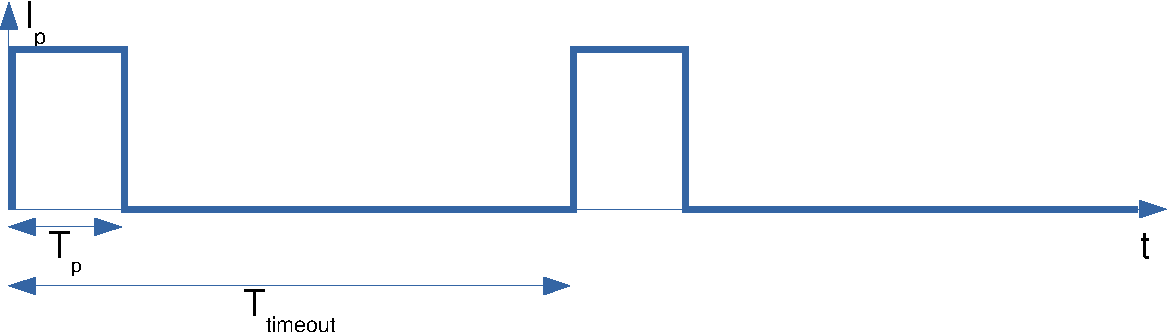
\includegraphics[width=\textwidth]{CapituloDDoS/Figuras/RTO_attack}
\caption{Ataque por retransmisión TCP}
\LABFIG{RTO attack} 
\end{figure}
%

\subsubsection{Ataque a Sistemas Operativos}\LABSSSEC{Ataques a SSOO}

El encargado de transportar correctamente los paquetes desde la red hasta la aplicación. Si el atacante es capaz de 
hacer que este intermediario no sea capaz de llevar los paquetes desde o hacia la aplicación, habrá logrado llevar a 
cabo un ataque \gls{DoS}.

En este tipo de ataque se busca explotar una vulnerabilidad en el modo que el \gls{SO} gestiona los paquetes. Por 
ejemplo, si a la hora de recibir un paquete, el \gls{SO} lo escribe en memoria sin comprobar los límites de la memoria 
reservada para ello, el atacante podría enviar un paquete lo suficientemente largo como para provocar un \emph{buffer 
overflow}\index{Buffer Overflow}, esto es, se escribirá en una zona de memoria indebida, provocando que el sistema 
colapse. Esta técnica es la empleada por el llamado \emph{ping de la muerte}\index{Ping de la Muerte}, ya explicado en 
el \SSSEC{DDoS semanticos}.

Otro ataque, también dirigido a saturar el \gls{SO}, sería un SYN flood (inundación SYN). Esta vez, con la inundación, 
no provocamos saturar la red, sino la capacidad de conexiones simultaneas que aguante el sistema.

\subsubsection{Ataques dirigidos a aplicaciones (Ataques capa 7)}

Muchas aplicaciones están desarrollando sus aplicaciones sobre una arquitectura tipo servicio web, esto es, programas 
distribuídos que funcionan mediante el paso de mensajes sobre el protocolo HTTP. Para que este servicio funcione, si 
está expuesto a internet, es necesario que el cortafuegos permita el tráfico hacia esa aplicación. Por tanto, el 
atacante es capaz también de alcanzar dicho servicio, aunque quizás no pueda usarlo por necesitar, por ejemplo, unas 
credenciales válidas.

Al igual que los servicios web, la aplicación distribuída puede estar confiando en cualquier otro tipo de tecnología 
subyacente. Mientras que esta se encuentre en espacio de usuario, se considerará un ataque de capa 7.

Los métodos para realizar este ataque son muy parecidos a los de la \SSSEC{Ataques a SSOO}. Por la parte semántica, se 
puede intentar enviar información corrupta que haga al servidor entrar en un estado incorrecto, que no pueda continuar 
sirviendo. Por otra parte, tenemos los ataques por inundación, que buscarían saturar la capacidad del servidor, y que 
a la máquina le sea imposible seguir respondiendo peticiones.


\section{Técnicas de detección y mitigacinó de un ataque DDoS}
\subsection{Ataques por inundación}
La principal señal que indica que un servicio está sufriendo un ataque por inundación es que reciben una cantidad de 
tráfico anormalmente grande. Sin embargo, para una detección correcta deberíamos definir qué supone \emph{anormal}. 

A lo largo de este trabajo intentaremos definir un sistema de detección de anomalías (CUSUM, \CHAP{TODO}), y qué 
parámetros debemos usar para buscar un compromiso entre velocidad de detección y no aparición de falsos positivos.

%TODO aún falta el tunning: Dificuktad de definir normal y anormal. Problemas de refinamiento.

Para mitigar el ataque, no basta con cortar el acceso al servicio, ya que entonces el \gls{DDoS} habría triunfado. Es 
necesario discernir entre las direcciones IP maliciosas o atacantes, y cortar el tráfico sólo a ellas, permitiendo que 
las direcciones benignas sigan navegando como hasta ahora.

\subsection{Ataques semánticos}
Para la detección de ataque ssemánticos, el método más usado es la detección de patrones. Esto es, analizar el paquete 
en busca de características del mismo que detecten que estamos ante un paquete, al menos sospechoso. Al patrón que 
siguen esos paquetes maliciosos y que, por tanto lo hace detectable, se le denomina \emph{firma}\index{Firma}.

Por ejemplo, en el caso del \emph{ping de la muerte}, un sistema intermedio podría analizar todos los paquetes que van 
hacia el servidor y, en caso de ser de un tamaño superior o igual a $2^16=65536$, bloquar el paso de dicho paquete.

Comparativamente hablando, tienen la desventaja de necesitar la constante actualización de la base de datos de firmas, 
y la posibilidad de que esta base de datos crezca, haciendose más inmanejable. Su refinamiento consiste en la selección 
de reglas adecuadas a los activos protegidos, esto es: Si no tengo un servidor web, no necesito estar analizando 
paquetes contra firmas que comprometen servidores web, es un gaso inútil.

Este es el sistema de detección usado por IPS tales como snort \cite{snort} o suricata \cite{suricata}. A lo largo de 
este trabajo no pretenderemos abarcar este tipo de soluciones.

\section{Resumen}%%%%%%%%%%%%%%%%%%%%%%%%%%%%%%%%%%%%%%%

\begin{Resumen}[Resumen del capítulo]
\subsection*{Definición}
Acción(es) que impiden que un sistema de información funcione normalmente.

\subsection*{Taxonomía}
\begin{align*}
 \begin{cases}
   \text{Por inundación.}
   \begin{cases}
     \text{Coordinados por seres humanos / manuales.}\\
     \qquad\text{\emph{Ningún elemento automático}}\\
     \text{Amplificados.}\\
     \qquad{\text{\emph{El atacante sólo envía N y el ataque se amplifica}}}\\
     \qquad{\text{\emph{Ejemplo: ping a direcciones broadcast}}}\\
     \text{Reflejados.}\\
     \qquad{\text{\emph{El atacante tiene una lista de IP que pueden reflejar su ataque}}}\\
     \qquad{\text{\emph{Ejemplo: Peticiones DNS con dirección origen de la víctima}}}\\
     \text{Botnets o redes Zombi.}\\
     \qquad{\text{\emph{Efecto amplificador y ocultador}}}
     \text{Combinación de las anteriores.}
   \end{cases}\\
   \text{Semántico.}\\
   \qquad{\text{\emph{Se busca explotar fallos}}}
 \end{cases}
\end{align*}

\subsection*{Objetivo del ataque}
\begin{align*}
 \begin{cases}
   \text{Dirigido a redes.}\\
   \qquad{\text{\emph{Ejemplos:}}}
   \begin{cases}
     \text{Reseteo de conexiones.} \\
     \text{Asentimientos optimistas.} \\
     \text{temporizador de retransmisión.} \\
   \end{cases}\\
   \text{Ataques a SSOO.} \\
   \text{Ataques de capa 7.}\\
 \end{cases}
\end{align*}

\subsection*{Técnicas de detección y mitigación}
\begin{align*}
 \begin{cases}
   \text{Por inundación.}
   \begin{cases}
     \text{Detección de comportamiento \emph{anómalo} en la red.} \\
     \qquad\rightarrow\text{¿Definición de anómalo?} \\
     \text{Bloqueo de direcciones con comportamientos anómalos}\\
     \qquad\rightarrow\text{Posibilidad de falsos negativos y falsos positivos}\\
     \text{Tuneado consistente en definir \emph{normal}}
   \end{cases}\\
   \text{Semánticos}
   \begin{cases}
     \text{Detección de patrones (firmas) en el tráfico.} \\
     \qquad\rightarrow\text{Necesidad de actualización} \\
     \text{Bloqueo de paquetes que cumplan dichos patrones}\\
     \qquad\rightarrow\text{Posibilidad de falsos negativos y falsos positivos} \\
     \text{Tuneado consiste en seleccionar reglas en base a los activos a proteger}
   \end{cases}\\
 \end{cases}
\end{align*}

\end{Resumen}


%
% !TEX root =../LibroTipoETSI.tex
\chapter{PF\_RING}\LABCHAP{PFRING}
\pagestyle{esitscCD}

\epigraph{In almost every computation a great variety of arrangements for the succession of the processes is possible, 
and various considerations must influence the selections amongst them for the purposes of a calculating engine. One 
essential object is to choose that arrangement which shall tend to reduce to a minimum the time necessary for completing 
the calculation.}{Ada Lovelace}

%\lettrine[lraise=0.7, lines=1, loversize=-0.25]{E}{l} 
\lettrine[lraise=-0.1, lines=2, loversize=0.25]{E}n un sistema de monitorización de tráfico, la captura de paquetes es 
un proceso vital. Si se quiere capturar tráfico a una velocidad aceptable, superiores a 1Gbps, es necesario que todo el 
proceso de captura de paquetes esté bien diseñado y sea eficiente. De no serlo, enseguida comenzaremos a notar 
pérdidas de paquetes, y nuestra monitorización no será efectiva.

%TODO unir con lo demás
Ya hemos cubierto la eficiencia en términos de procesamiento de paquetes en los anteriores capítulos. 

\gls{PFRING} es, según su autor Luca Deri, una tecnología que persigue capturar tráfico a $10G$ sin necesitar tarjetas 
especializadas, sin pérdidas y bajo cualquier circunstancia del tráfico, de forma que sea posible crear sondas de 
tráfico software con el mismo rendimiento que las basadas en hardware \cite{LucaDeriPFRING}.

A lo largo de este capítulo, %TODO

\section{Proceso de paquetes por el núcleo linux}\LABSEC{sec:ProcesoPaquetesLinux}
El paso de paquetes a través del núcleo Linux puede ser un importante cuello de botella. %TODO ampliar

\subsection{Reserva de memoria para almacenar el paquete}
El primer paso en la recepción de paquetes es que éste llegue a la tarjeta de red a través de la interfaz física. Tan 
pronto como esto ocurre, y la memoria interna de la \gls{NIC} contiene el paquete completo, ésta es responsable de 
de crear una estructura de datos para almacenar el paquete en la memoria principal del sistema, y copiarlo ahí.

Esta reserva ya incluye un corte en términos de tiempo, ya que dos procesos no pueden reservar memoria al mismo tiempo. 
El sistema tiene una tabla de memoria en la que están anotados los distintos bloques que cada proceso (incluído el 
núcleo) tiene reservada. Si dos procesos reservasen al mismo tiempo, podría ocurrir que reservasen segmentos de memoria 
solapados.

Por tanto, la reserva debe ser sincronizada, y esta sincronización consume un tiempo importante. Tras ello, la copia es 
en modo \gls{DMA}, por lo que la tarjeta obtiene acceso exclusivo a esa memoria y no es necesario la intervención de la 
CPU para copiar los datos.

El paquete es entonces copiado en una estructura de datos \texttt{sk\_buff}. Dicha estructura es bastante grande, y 
puede ir creciendo a medida que lo necesita. Esto incrementa la fragmentación de memoria, ya que al crecer es posible 
que no quepa en su segmento de memoria, y deba moverse a otro segmento mayor.

Por último, existen bastantes datos de la estructura que son privados, y no deben viajar de una capa a otra en el paso 
de información. Por tanto, hay que clonar la estructura al transmitir información\footnote{Si bien hay partes de la 
misma que pueden mantenerse}, lo que redunda en más reservas y más retrasos por sincronía
\cite{skBuffLinuxFoundation}.

\subsection{Notificación del nuevo paquete}
Cuando el paquete al completo es copiado en la memoria principal, es necesario un mecanismo de notificación al 
\gls{controlador}\index{Controlador de Dispositivo} de red de Linux para que éste pueda procesarlo. Se usa, entonces, 
una interrupción hardware.

La interrupción provoca que el núcleo deje de realizar las tareas que esté haciendo para hacer caso a la llegada del 
paquete. Sin embargo, si tenemos demasiados paquetes por segundo, no dejamos a Linux avanzar, y destrozamos la 
planificación de tareas. Este hecho es conocido como Tormenta de Interrupciones\index{Tormenta de Interrupciones} o 
\emph{interrupt storm} \cite{p206}.

En cada interrupción, la función llamada es \texttt{netif\_rx} o \texttt{netif\_receive\_skb}.

\subsubsection{NAPI}
Para evitar la tormenta de interrupciones, se pueden utilizar técnicas como la llamada \emph{device polling}. El 
funcionamiento es el siguiente \cite{beyondDevicePolling}.
\begin{itemize}
 \item Cuando un nuevo paquete llega, la tarjeta genera una interrupción.
 \item El \gls{SO} la maneja de la siguiente forma:
 \begin{enumerate}
  \item Prohíbe (enmascara) futuras interrupciones del dispositivo.
  \item Programa una tarea para atender a la tajeta en un futuro.
  \item Cuando la atiende, levanta la prohibición de interrupciones.
 \end{enumerate}
\end{itemize}

La implementación de esta técnica en Linux es conocida como \gls{NAPI}.

Podemos ver en las figuras \FIG{InterrupcionesNIC} y \FIG{DevicePolling} las diferencias entre un canal saturado 
con un método y otro. Se observa como, en la primera figura, al núcleo no le da tiempo a procesar todos los paquetes 
del canal saturado, y sólo puede procesar una de cada dos. Sin embargo, en la segunda figura, Linux procesa los 
paquetes cuando puede, en tiempos aleatorios, y coge de una tacada todos los paquetes que necesita.

\begin{figure}[hbtp]
\centering
%\hfill
\subfloat[Interrupción]%
   {\LABFIG{InterrupcionesNIC}%
   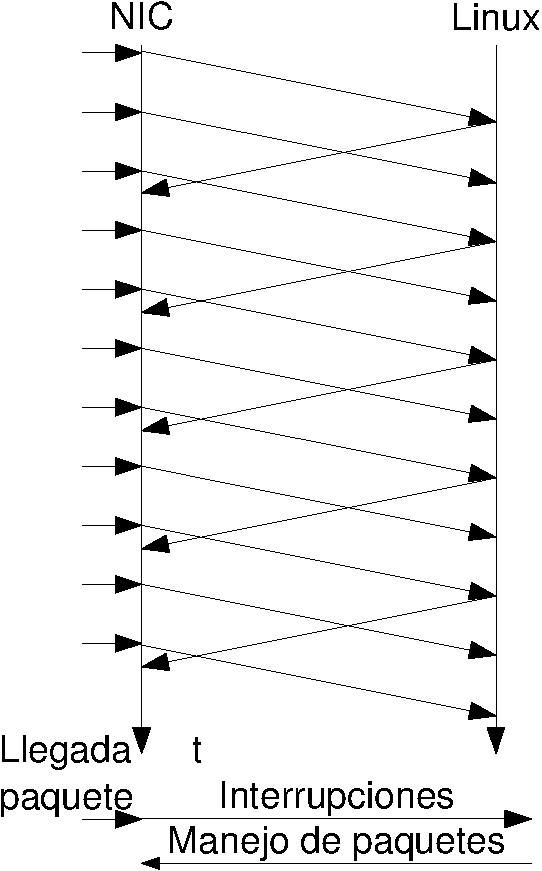
\includegraphics[width=0.30\textwidth]{CapituloPF_RING/Figuras/InterrupcionesNIC-crop}}%
\hspace{0.2\textwidth}
\subfloat[Device Polling]%
 {\LABFIG{DevicePolling}%
 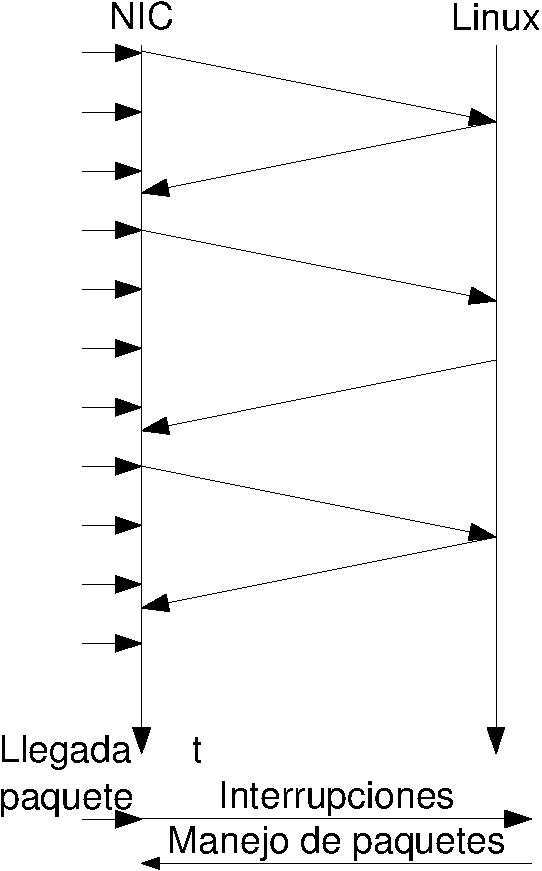
\includegraphics[width=0.30\textwidth]{CapituloPF_RING/Figuras/PollNIC-crop}}%
%
\caption{Comparativa entre los diferentes métodos de notificación de nuevos paquetes}
\end{figure}
%

\subsection{Obtención del paquete por parte del kernel}
Una interrupción debe ser rápida, esto es, en una interrupción no podemos realizar tareas que no sean estrictamente 
necesarias, por las mismas razones que las señales en espacio de usuario. Por ello, la interrupción provoca que se 
planee una tarea con el fin de recoger el paquete.

A partir de ese momento, sólo cuando el planeador decida que el sistema está libre, se recogerá el / los paquetes 
usando \texttt{packet\_rcv}, y se pasará a la pila de red de Linux.

En la pila, el paquete pasará por diversos sistemas, como la parte de filtrado 
\emph{\gls{netfilter}}\index{Netfilter} para, finalmente, ser recibido por un puerto o \emph{\gls{socket}} llegar a 
estar listo para la recogida por parte del espacio de usuario \cite{p206}.

\subsection{Obtención del paquete por parte del espacio de usuario}
La recepción de paquetes en el espacio de usuario se realiza mediante la librería \emph{\gls{libpcap}}\index{libpcap}.
Para ello, \emph{\gls{libpcap}} genera un \emph{\gls{socket}} que es abstraído por un descriptor de fichero. Si 
aplicamos la llamada al sistema \texttt{select} o \texttt{poll}, podemos saber si el socket dispone de datos para ser 
leídos, y leerlos en ese caso con la llamada \texttt{recvfrom}.

Un ejemplo de este tipo de lecturas podemos verlo en en \lstlistingname{}\ref{code:lecturaRawSocket}. En él, vemos la 
creación del socket con \texttt{socket}, la consulta de disponibilidad con \texttt{poll} y la recepción de los datos 
con \texttt{recvfrom}.

\begin{lstlisting}[language=C++,caption={Lectura desde un socket crudo}, 
breaklines=true, label=code:lecturaRawSocket,numbers=left,float=htbp]
#include<stdio.h>
#include<string.h>

#include<net/ethernet.h>
#include<sys/socket.h>
#include<arpa/inet.h>
#include<sys/ioctl.h>
#include<sys/types.h>
 
void ProcessPacket(char* , int);
 
int main(){
    size_t saddr_size, data_size;
    struct sockaddr saddr;
         
    char buffer[65536];
   
    int sock_raw = socket(AF_PACKET, SOCK_RAW, htons(ETH_P_ALL));
    setsockopt(sock_raw, SOL_SOCKET, SO_BINDTODEVICE, "eth0", 
                                               strlen("eth0")+1);
     
    if(sock_raw < 0){
        perror("Socket Error");
        return 1;
    }
    while(1){
        struct pollfd fds = { fd: sock_raw, events: POLLIN};
        const int poll_rc = poll(&fsd, 1, 1000);
        if(poll_rc == 0){
            if(poll_rc <= 0)
                perror("Poll error");
            continue;
        }
        saddr_size = sizeof(saddr);
        //Receive a packet
        data_size = recvfrom(sock_raw, buffer, 65536, 0, &saddr, 
                                       (socklen_t*)&saddr_size);
        if(data_size < 0){
            printf("Recvfrom error , failed to get packets\n");
            return 1;
        }
        //Now process the packet
        ProcessPacket(buffer , data_size);
    }
    close(sock_raw);
    return 0;
}
\end{lstlisting}

Sin embargo, este procedimiento tiene un coste oculto. A la hora de leer los datos, estos son copiados desde la 
memoria del núcleo a un buffer en espacio de usuario. Esto es, por cada paquete, estamos perdiendo tiempo y ciclos de 
CPU en copiar un dato que sólo vamos a leer.

Si, por ejemplo, queremos leer paquetes de 150kb en un enlace saturado a una velocidad de 1Gbps, estamos realizando:
\begin{itemize}
 \item $\frac{1G}{150k} \approx 7000$ llamadas al sistema con \texttt{poll} y otras tantas con \texttt{recvfrom}.
 \item Copiando entre regiones de memoria RAM a 1Gbps.
\end{itemize}

\section{La alternativa: PF\_RING}\LABSEC{La alternativa: PF RING}


\endinput

\begin{Resumen}[Resumen de PF RING]


\subsection*{S1}

\end{Resumen}


% 
%%:Empezamos con los apéndices, que irían en uno o más ficheros. Es necesario incluir estos ficheros entre el entorno \begin{appendices}....\end{appendices} debido a que se ha deseado utilizar un formato diferente para el título de los apéndices, incluyendo la palabra apéndice, para la numeración de los apéndices, alfabético, y para las cabeceras de las páginas.
%
%\begin{appendices}
%
%% Fichero en el que se incluyen los apéndices
%% !TEX root =../LibroTipoETSI.tex



%APENDICE A
\chapter{Sobre  \LaTeX}\LABAPEN{ApA}
{Este es un ejemplo de apéndices, el texto es únicamente relleno, para que el lector pueda observar cómo se utiliza}
%%%%%%%%%%%%%%%%%
\section{Ventajas de \LaTeX}

El gusto por el \LaTeX\ depende de la forma de trabajar de cada uno. La principal virtud es la facilidad de formatear cualquier texto y la robustez. Incluir títulos, referencias es inmediato.
%\Blindtext
%\lipsum
Las ecuaciones quedan estupendamente, como puede verse en \EQ{Ap1}
\begin{equation}\LABEQ{Ap1}
x_{1}=x_{2}.
\end{equation}


\section{Inconvenientes}
%\Blindtext
El principal inconveniente de \LaTeX\ radica en la necesidad de aprender un conjunto de comandos para generar los elementos que queremos. Cuando se está acostumbrado a un entorno ``como lo escribo se obtiene'', a veces resulta difícil dar el salto a ``ver'' que es lo que se va a obtener con un determinado comando. 

Por otro lado, en general será muy complicado cambiar el formato para desviarnos de la idea original de sus creadores. No es imposible, pero sí muy difícil. Por ejemplo, con la sentencia siguiente:
 
\begin{lstlisting}[language=,caption={Escritura de una ecuación}, breaklines=true, label=prgA1-01]
\begin{equation}\LABEQ{Ap2}
x_{1}=x_{2}
\end{equation}
\end{lstlisting}
obtenemos:
\begin{equation}\LABEQ{Ap2}
x_{1}=x_{2}
\end{equation}
Esto será siempre así. Aunque, tal vez, esto podría ser una ventaja y no un incoonveniente.

Para una discusión similar sobre el Word\tsp{\textregistered}, ver \APEN{ApB}.
%\Blindtext


%%%%%%%%%%%%%%%%%%%%%%%%%%%%%%%%%%%%%%%
%APENDICE B
\chapter{Sobre Microsoft Word\tsp{\textregistered}}\LABAPEN{ApB}

\section{Ventajas del Word\tsp{\textregistered}}
La ventaja mayor del Word\tsp{\textregistered} es que permite configurar el formato muy fácilmente. Para las ecuaciones,
\begin{equation}
x_{1}=x_{2},
\end{equation}
tradicionalmente ha proporcionado pésima presentación. Sin embargo, el software adicional Mathtype\tsp{\textregistered} solventó este problema, incluyendo una apariencia muy profesional y cuidada. Incluso permitía utilizar un estilo similar al \LaTeX\xspace. Además, aunque el Word\tsp{\textregistered} incluye sus propios atajos para escribir ecuaciones,  Mathtype\tsp{\textregistered} admite también escritura \LaTeX\xspace. En las últimas versiones de Word\tsp{\textregistered}, sin embargo, el formato de ecuaciones está muy cuidado, con un aspecto similar al de \LaTeX.


\section{Inconvenientes de Word\tsp{\textregistered}}
Trabajar con títulos, referencias cruzadas e índices es un engorro, por no decir nada sobre la creación de una tabla de contenidos. Resulta muy frecuente que alguna referencia quede pérdida o huérfana y aparezca un mensaje en negrita indicando que  no se encuentra. 

Los estilos permiten trabajar bien definiendo la apariencia, pero también puede desembocar en un descontrolado incremento de los mismos. Además, es muy probable que Word\tsp{\textregistered} se quede colgado, sobre todo al trabajar con copiar y pegar de otros textos y cuando se utilizan ficheros de gran extensión, como es el caso de un libro.

%\end{equation}
 %Ver este fichero para incluir ahí los apéndices.
%
%\end{appendices}
%:Fin de la inclusión de apéndices

%:Empieza todo lo que no constituye el cuerpo en si del libro. Todo lo que va detrás
\backmatter

%:Indice de figuras, coméntese las siguientes líneas si no se desea
\cleardoublepage
\phantomsection

%:Para añadir una línea en blanco en el TOC y separar esta lista
\addtocontents{toc}{\protect\mbox{}\protect\hspace*{0pt}\par}
\addcontentsline{toc}{listasb}{\listfigurename}
\pagestyle{especial}
\listoffigures

%:Indice de tablas, coméntese las siguientes líneas si no se desea
\cleardoublepage
\phantomsection
\addcontentsline{toc}{listasb}{\listtablename}
\pagestyle{especial}
\listoftables

%:Indice de Programas
\cleardoublepage
\phantomsection
\addcontentsline{toc}{listasb}{\lstlistlistingname}
\pagestyle{especial}
\lstlistoflistings

%:Bibliografía con biblatex y biber
\cleardoublepage
\phantomsection
\addcontentsline{toc}{listasb}{\bibname}
\pagestyle{especial}
%BIBER
%\printbibliography[heading=etsi]La mecánica del a
%BIBTEX
%\bibliographystyle{IEEEtran}
\bibliographystyle{amsplain} %flexbib amsplain alpha
%:Fichero con la bibliografía, BIBTEX
\bibliography{bibliografiaLibroETSI}

%:Índice alfabético de palabras
\cleardoublepage
\phantomsection
\addcontentsline{toc}{listasb}{\indexname}
\chaptermark{\indexname}
\printindex


%:Acrónimos
\cleardoublepage
\phantomsection
\addcontentsline{toc}{listasb}{\glossaryname}
\chaptermark{\glossaryname}
\printglossaries

\end{document}